\documentclass[11pt,a4paper,]{article}
\usepackage{lmodern}

\usepackage{amssymb,amsmath}
\usepackage{ifxetex,ifluatex}
\usepackage{fixltx2e} % provides \textsubscript
\ifnum 0\ifxetex 1\fi\ifluatex 1\fi=0 % if pdftex
  \usepackage[T1]{fontenc}
  \usepackage[utf8]{inputenc}
\else % if luatex or xelatex
  \usepackage{unicode-math}
  \defaultfontfeatures{Ligatures=TeX,Scale=MatchLowercase}
\fi
% use upquote if available, for straight quotes in verbatim environments
\IfFileExists{upquote.sty}{\usepackage{upquote}}{}
% use microtype if available
\IfFileExists{microtype.sty}{%
\usepackage[]{microtype}
\UseMicrotypeSet[protrusion]{basicmath} % disable protrusion for tt fonts
}{}
\PassOptionsToPackage{hyphens}{url} % url is loaded by hyperref
\usepackage[unicode=true]{hyperref}
\hypersetup{
            pdftitle={Determining Factors for 10 year-Local Currency Bonds: Indonesia Case},
            pdfborder={0 0 0},
            breaklinks=true}
\urlstyle{same}  % don't use monospace font for urls
\usepackage{geometry}
\geometry{a4paper, centering, text={16cm,24cm}}
\usepackage[style=authoryear-comp,]{biblatex}
\addbibresource{baca.bib}
\usepackage{longtable,booktabs}
% Fix footnotes in tables (requires footnote package)
\IfFileExists{footnote.sty}{\usepackage{footnote}\makesavenoteenv{long table}}{}
\usepackage{graphicx,grffile}
\makeatletter
\def\maxwidth{\ifdim\Gin@nat@width>\linewidth\linewidth\else\Gin@nat@width\fi}
\def\maxheight{\ifdim\Gin@nat@height>\textheight\textheight\else\Gin@nat@height\fi}
\makeatother
% Scale images if necessary, so that they will not overflow the page
% margins by default, and it is still possible to overwrite the defaults
% using explicit options in \includegraphics[width, height, ...]{}
\setkeys{Gin}{width=\maxwidth,height=\maxheight,keepaspectratio}
\IfFileExists{parskip.sty}{%
\usepackage{parskip}
}{% else
\setlength{\parindent}{0pt}
\setlength{\parskip}{6pt plus 2pt minus 1pt}
}
\setlength{\emergencystretch}{3em}  % prevent overfull lines
\providecommand{\tightlist}{%
  \setlength{\itemsep}{0pt}\setlength{\parskip}{0pt}}
\setcounter{secnumdepth}{5}

% set default figure placement to htbp
\makeatletter
\def\fps@figure{htbp}
\makeatother


\title{Determining Factors for 10 year-Local Currency Bonds: Indonesia Case}

%% MONASH STUFF

%% CAPTIONS
\RequirePackage{caption}
\DeclareCaptionStyle{italic}[justification=centering]
 {labelfont={bf},textfont={it},labelsep=colon}
\captionsetup[figure]{style=italic,format=hang,singlelinecheck=true}
\captionsetup[table]{style=italic,format=hang,singlelinecheck=true}


%% FONT
\RequirePackage{bera}
\RequirePackage[charter,expert,sfscaled]{mathdesign}
\RequirePackage{fontawesome}

%% HEADERS AND FOOTERS
\RequirePackage{fancyhdr}
\pagestyle{fancy}
\rfoot{\Large\sffamily\raisebox{-0.1cm}{\textbf{\thepage}}}
\makeatletter
\lhead{\textsf{\expandafter{\@title}}}
\makeatother
\rhead{}
\cfoot{}
\setlength{\headheight}{15pt}
\renewcommand{\headrulewidth}{0.4pt}
\renewcommand{\footrulewidth}{0.4pt}
\fancypagestyle{plain}{%
\fancyhf{} % clear all header and footer fields
\fancyfoot[C]{\sffamily\thepage} % except the center
\renewcommand{\headrulewidth}{0pt}
\renewcommand{\footrulewidth}{0pt}}

%% MATHS
\RequirePackage{bm,amsmath}
\allowdisplaybreaks

%% GRAPHICS
\RequirePackage{graphicx}
\setcounter{topnumber}{2}
\setcounter{bottomnumber}{2}
\setcounter{totalnumber}{4}
\renewcommand{\topfraction}{0.85}
\renewcommand{\bottomfraction}{0.85}
\renewcommand{\textfraction}{0.15}
\renewcommand{\floatpagefraction}{0.8}


%\RequirePackage[section]{placeins}

%% SECTION TITLES


%% SECTION TITLES
\RequirePackage[compact,sf,bf]{titlesec}
\titleformat*{\section}{\Large\sf\bfseries\color[rgb]{0.7,0,0}}
\titleformat*{\subsection}{\large\sf\bfseries\color[rgb]{0.7,0,0}}
\titleformat*{\subsubsection}{\sf\bfseries\color[rgb]{0.7,0,0}}
\titlespacing{\section}{0pt}{2ex}{.5ex}
\titlespacing{\subsection}{0pt}{1.5ex}{0ex}
\titlespacing{\subsubsection}{0pt}{.5ex}{0ex}


%% TITLE PAGE
\def\Date{\number\day}
\def\Month{\ifcase\month\or
 January\or February\or March\or April\or May\or June\or
 July\or August\or September\or October\or November\or December\fi}
\def\Year{\number\year}

%% LINE AND PAGE BREAKING
\sloppy
\clubpenalty = 10000
\widowpenalty = 10000
\brokenpenalty = 10000
\RequirePackage{microtype}

%% PARAGRAPH BREAKS
\setlength{\parskip}{1.4ex}
\setlength{\parindent}{0em}

%% HYPERLINKS
\RequirePackage{xcolor} % Needed for links
\definecolor{darkblue}{rgb}{0,0,.6}
\RequirePackage{url}

\makeatletter
\@ifpackageloaded{hyperref}{}{\RequirePackage{hyperref}}
\makeatother
\hypersetup{
     citecolor=0 0 0,
     breaklinks=true,
     bookmarksopen=true,
     bookmarksnumbered=true,
     linkcolor=darkblue,
     urlcolor=blue,
     citecolor=darkblue,
     colorlinks=true}

\usepackage[showonlyrefs]{mathtools}
\usepackage[no-weekday]{eukdate}

%% BIBLIOGRAPHY

\makeatletter
\@ifpackageloaded{biblatex}{}{\usepackage[style=authoryear-comp, backend=biber, natbib=true]{biblatex}}
\makeatother
\ExecuteBibliographyOptions{bibencoding=utf8,minnames=1,maxnames=3, maxbibnames=99,dashed=false,terseinits=true,giveninits=true,uniquename=false,uniquelist=false,doi=false, isbn=false,url=true,sortcites=false}

\DeclareFieldFormat{url}{\texttt{\url{#1}}}
\DeclareFieldFormat[article]{pages}{#1}
\DeclareFieldFormat[inproceedings]{pages}{\lowercase{pp.}#1}
\DeclareFieldFormat[incollection]{pages}{\lowercase{pp.}#1}
\DeclareFieldFormat[article]{volume}{\mkbibbold{#1}}
\DeclareFieldFormat[article]{number}{\mkbibparens{#1}}
\DeclareFieldFormat[article]{title}{\MakeCapital{#1}}
\DeclareFieldFormat[article]{url}{}
%\DeclareFieldFormat[book]{url}{}
%\DeclareFieldFormat[inbook]{url}{}
%\DeclareFieldFormat[incollection]{url}{}
%\DeclareFieldFormat[inproceedings]{url}{}
\DeclareFieldFormat[inproceedings]{title}{#1}
\DeclareFieldFormat{shorthandwidth}{#1}
%\DeclareFieldFormat{extrayear}{}
% No dot before number of articles
\usepackage{xpatch}
\xpatchbibmacro{volume+number+eid}{\setunit*{\adddot}}{}{}{}
% Remove In: for an article.
\renewbibmacro{in:}{%
  \ifentrytype{article}{}{%
  \printtext{\bibstring{in}\intitlepunct}}}

\AtEveryBibitem{\clearfield{month}}
\AtEveryCitekey{\clearfield{month}}

\makeatletter
\DeclareDelimFormat[cbx@textcite]{nameyeardelim}{\addspace}
\makeatother

\author{{\sf\Large\textbf{ Avega Editya}\\\sf\large Nobel Prize, PhD\\[0.5cm]}{\sf\Large\textbf{ Pierre Curie}\\\sf\large Nobel Prize, PhD\\[0.5cm]}

\date{\sf\Date~\Month~\Year}
\makeatletter
\lfoot{\sf Editya, Curie: \@date}
\makeatother


%%%% PAGE STYLE FOR FRONT PAGE OF REPORTS

\makeatletter
\def\organization#1{\gdef\@organization{#1}}
\def\telephone#1{\gdef\@telephone{#1}}
\def\email#1{\gdef\@email{#1}}
\makeatother
  \organization{Monash Business School}

  \def\name{Department of\newline Econometrics \&\newline Business Statistics}

  \telephone{(03) 9905 2478}

  \email{\href{mailto:mcurie.notreal@gmail.com}{\nolinkurl{mcurie.notreal@gmail.com}}}

\def\webaddress{\url{http://buseco.monash.edu/ebs/consulting/}}
\def\abn{12 377 614 012}
\def\logo{
\includegraphics[width=6cm]{MBSportrait}}
\def\extraspace{\vspace*{1.6cm}}
\makeatletter
\def\contactdetails{\faicon{phone} & \@telephone \\
                    \faicon{envelope} & \@email}
\makeatother

%%%% FRONT PAGE OF REPORTS

\def\reporttype{Report for}

\long\def\front#1#2#3{
\newpage
\begin{singlespacing}
\thispagestyle{empty}
\vspace*{-1.4cm}
\hspace*{-1.4cm}
\hbox to 16cm{
  \hbox to 6.5cm{\vbox to 14cm{\vbox to 25cm{
    \logo
    \vfill
    \parbox{6.3cm}{\raggedright
      \sf\color[rgb]{0.00,0.00,0.70}
      {\large\textbf{\name}}\par
      \vspace{.7cm}
      \tabcolsep=0.12cm\sf\small
      \begin{tabular}{@{}ll@{}}\contactdetails
      \end{tabular}
      \vspace*{0.3cm}\par
      ABN: \abn\par
    }
  }\vss}\hss}
  \hspace*{0.2cm}
  \hbox to 1cm{\vbox to 14cm{\rule{1pt}{26.8cm}\vss}\hss\hfill}
  \hbox to 10cm{\vbox to 14cm{\vbox to 25cm{
      \vspace*{3cm}\sf\raggedright
      \parbox{11cm}{\sf\raggedright\baselineskip=1.2cm
         \fontsize{24.88}{30}\color[rgb]{0.70,0.00,0.00}\sf\textbf{#1}}
      \par
      \vfill
      \large
      \vbox{\parskip=0.8cm #2}\par
      \vspace*{2cm}\par
      \reporttype\\[0.3cm]
      \hbox{#3}%\\[2cm]\
      \vspace*{1cm}
      {\large\sf\textbf{\Date~\Month~\Year}}
   }\vss}
  }}
\end{singlespacing}
\newpage
}

\makeatletter
\def\titlepage{\front{\expandafter{\@title}}{\@author}{\@organization}}
\makeatother

\usepackage{setspace}
\setstretch{1.5}

%% Any special functions or other packages can be loaded here.
\usepackage{booktabs}
\usepackage{longtable}
\usepackage{array}
\usepackage{multirow}
\usepackage{wrapfig}
\usepackage{float}
\usepackage{colortbl}
\usepackage{pdflscape}
\usepackage{tabu}
\usepackage{threeparttable}
\usepackage{threeparttablex}
\usepackage[normalem]{ulem}
\usepackage{makecell}
\usepackage{xcolor}


\begin{document}
\titlepage

\newpage

\hypertarget{introduction}{%
\section{Introduction}\label{introduction}}

Indonesian government regularly issue Rupiah-denominated sovereign bonds (conventional and sharia bonds) in the primary market to finance the deficit of the national budget. In 2021, the issuance target for the sovereign bonds is around 80-85\% of total deficit financing which amounts to IDR1,006 Trillion or equivalent to USD72 Billion \footnote{Assumed exchange rate for conversion (IDR/USD) = 14,284.00}. As of 2 September 2021, the total outstanding of local currency sovereign bonds (LCB) is IDR4,539 Trillion or equivalent to USD318 billion \footnote{ibid}.

The government sells the sovereign bonds through an auction which is conducted every Tuesday. The announcement will be released three days before the auction day (T-3). During a 2-hour auction, investors (both individuals and institutions) can put their bidding in multiple prices through primary dealers, and auction winners will pay their bonds based on their proposed volumes and yields. In addition to the multiple price (competitive) mechanism, the government also offers LCB to several non-competitive participants such as Indonesia Central Bank (Bank Indonesia) and Indonesia Deposit Insurance Corporation (Lembaga Penjamin Simpanan). This non-competitive buying may also be conducted by primary dealers to complement their competitive bidding purchase. Non-competitive buyers will pay their LCB based on weighted average yield (WAY) from the winning competitive bidding.

There are several benchmark series of LCB offered in the auction. These series represent various maturity times. For conventional bonds, tenors of benchmark series in 2021 are ranging from 5, 10, 15, and 20 years. Meanwhile, benchmark tenors of sharia bonds cover 2, 4, 13, and 25 years.

Since 2021, the yield of 10-year LCB has become one of the macroeconomic assumptions in the national budget, replacing treasury bills of tenor 3-month (Surat Perbendaharaan Negara). This replacement is because the yield of 10-year LCB is deemed as having a larger and more significant portion in the nation's cost of borrowing compared to the T-bills. Moreover, the 10-year yield is also reflecting long-term economic development and its movement is commonly used as a sign for predicting country's economic health.

During a period of 2014-2018, Indonesia is said to have a higher average of 10-year sovereign bonds yield compared to its ASEAN-5 peers (Thailand, Philippines, Malaysia, Vietnam) as well as several other emerging countries with similar credit ratings like Mexico, Columbia, and India \autocite{Muktiyanto2019}. This condition makes Indonesia pays more expensive debt compared to these countries. As corporate and business use the yield for benchmarking when issuing their LCB as well as lending money, the impact of costly debt is also spilled over in the national economy.

Considering the important functions of the 10-year LCB yield in Indonesia's economy, this study will analyze several variables that determine the yield and quantify their impact using the Ordinary Least Squared (OLS) model. This paper will be delivered in several sections. First, we will explain our research's purpose in Section 2. Section 3 will provide background knowledge from prior studies and explanation of the collected data. Section 4 will focus on exploratory data analysis (EDA) by visualizing data to check any interesting features of the variables. Section 5 and section 6 will cover the research methodology and result of analysis subsequently. The Appendix contains additional information.

\hypertarget{motivation}{%
\section{Motivation}\label{motivation}}

This paper provides two new values to existing literature. First, it employs an exploratory data analysis (EDA) approach at the beginning of analysis to gain better intuition of each explanatory variable. This approach is quite important especially for capturing particular data characteristics, i.e.~non-linearity before we can proceed to a confirmatory step. Disregarding the data characteristic will result in inappropriate data modeling.
Second, this is the first work that empirically studies the impact of primary dealers' behavior on the 10-year LCB yield in Indonesia.\\
The purpose of this work will be to provide insights and policy recommendations for the government in reducing LCB yield, particularly by aiming at significant determinant factors, which in turn help to optimize the national's cost of borrowing.

\hypertarget{explanation-of-collected-data}{%
\section{Explanation of Collected Data}\label{explanation-of-collected-data}}

There are 7 variables used in this paper as explanatory variables to the Indonesia's LCB yield; US Treasury (UST) yield, Credit Default Swap (CDS), foreign ownership (\%), central bank's policy rate (policy rate), exchange rate, volatility index (VIX) and a dummy variable of auction/non-auction days as a proxy to primary dealers' trading behavior. The use of these explanatory variables are following numerous studies that have been conducted previously by various authors.

The UST yield is said by \autocite{Miyajima2015} and \autocite{Muktiyanto2019} to be significantly affecting bonds yield. Miyajima et al. \autocite*{Miyajima2015} conclude that the UST yield, while not a main contributor to the LCB yield in the emerging economies, is to some extent affecting the yield. Muktiyanto et al.~whose focus of study is on Indonesia's bonds gives more emphasize on the predictor variable suggesting that the UST yield is not only significant but also has the biggest role in determining the LCB yield of the country. On the contrary, Permanasari et al. \autocite*{Permanasari2021} who also study the same country suggest that the UST yield has no significant effect in determining the LCB yield.

Furthermore, Kim et. al \autocite*{Kim2014} and Muktiyanto et al. \autocite*{Muktiyanto2019} find that Credit Default Swap (CDS) is a significant factor that affecting the yield. The first name, using yield spread decomposition approach, suggest that the CDS as a proxy to default risk has 37\% contribution to the spread. Muktiyanto et al. \autocite{Muktiyanto2019} support this finding by suggesting the significant effect of the CDS on the Indonesia's LCB yield.

The effect of foreign ownership on the bonds yield is studied by researchers like Gadanecz et al. \autocite*{Gadanecz2018} who confirm the significance of the variable in LCB market. Another study with similar tone by Dachroui et al. \autocite{Dachraoui2020} who analyze role of capital flight as a driver of sovereign bonds spreads in Latin American countries, conclude that the spreads are positively correlated with the capital flight \autocite*{Dachraoui2020}.

Our fourth predictor variables used in this study, the policy rate, is inspired by findings from several works in Indonesia conducted by Muktiyanto et al. \autocite*{Muktiyanto2019} and Kurniasih et al. \autocite*{Kurniasih2015} These authors analyze relationship between the predictor with Indonesia's bonds yield. Both studies agree that the policy rate significantly affect the yield in a positive direction.

Moreover, some works highlight the effect of exchange rate on the bonds yield \autocite{Miyajima2015}, \autocite{Gadanecz2018}, \autocite{Saenong2020} and \autocite{Permanasari2021}. Miyajima et al. \autocite*{Miyajima2015} suggest crucial effect of the exchange rate on the yield in emerging economies, while Gadanecz et al \autocite{Gadanecz2018} using exchange rate volatility and expected exchange rate as predictor variables also confirm the significant relationship. These two studies are inline with a work by Permanasari et al. \autocite*{Permanasari2021} who study the effect on Indonesia's bonds yield, suggesting significant negative-relationship between the exchange rate and the yield. A slight different conclusion is provided by Saenong et al \autocite{Saenong2020} who argue that the effect on the Indonesia's bonds yield only significant in the short run but find to be insignificant in the long run.

Meanwhile, relationship between our sixth predictor-the VIX and the bonds yield is said to be significant by several researchers like \autocite{Miyajima2015}, \autocite{Izadi2018}, and \autocite{Dachraoui2020}. Miyajima find the significant relationship in several emerging market being observed, while Izadi et al. \autocite{Izadi2018} also find the similar effect in all 24 developed countries in
North America, Europe and Pacific Rim regions. In addition, Dachraoui \autocite*{Dachraoui2020} confirm the significant effect in Latin America.

Other researches like Tchuindjo et al.\autocite*{Tchuindjo2015}, Endo \autocite*{Endo2020}, Nyborg et al. \autocite*{Nyborg2004}, Mercer et al. \autocite*{Mercer2013}, and Ferrari et al. \autocite*{Ferrari2018} took different angle by looking at primary dealers system and its impact on bonds yield. Endo \autocite*{Endo2020} study role of primary dealers in low income economies, while Ferrari et al. \autocite*{Ferrari2018} focus on primary dealers' funding constraints on sovereign bonds yield. Nyborg et al. \autocite*{Nyborg2004}, Mercer et al. \autocite*{Mercer2013} and Tchuindjo \autocite*{Tchuindjo2015} concern on primary dealers trading behavior in US Treasury auction. The last name also provide several mathematical models to estimate the impact of primary dealers' strategic behavior in the auction \autocite*{Tchuindjo2015}.

For the purpose of our study, we will use 10-year US Treasury (UST) yield, 5-year Indonesia's Credit Default Swap (CDS), foreign ownership in Indonesia's 10-year bonds(\%), Bank Indonesia's policy rate, exchange rate (IDR/USD), Indonesia's volatility index (VIX) as well as a dummy variable of Indonesian government auction days as a proxy of Indonesia's primary dealers' behavior. Our response variable is the 10-year Indonesia's LCB yield. All variables are collected as time-series data covering period from 2 January 2015 up to 5 August 2021 and can be described as follow:

\hypertarget{year-lcb-yield}{%
\subsection{10-year LCB Yield}\label{year-lcb-yield}}

Yield is expected return demanded by investors as exchange of risks being borne. The 10-year yield data used in this study is a Indonesia's generic yield retrieved from Bloomberg platform using ticker code ``GRR'' (global summary of government bill, note, and benchmark bond rates for individual countries).

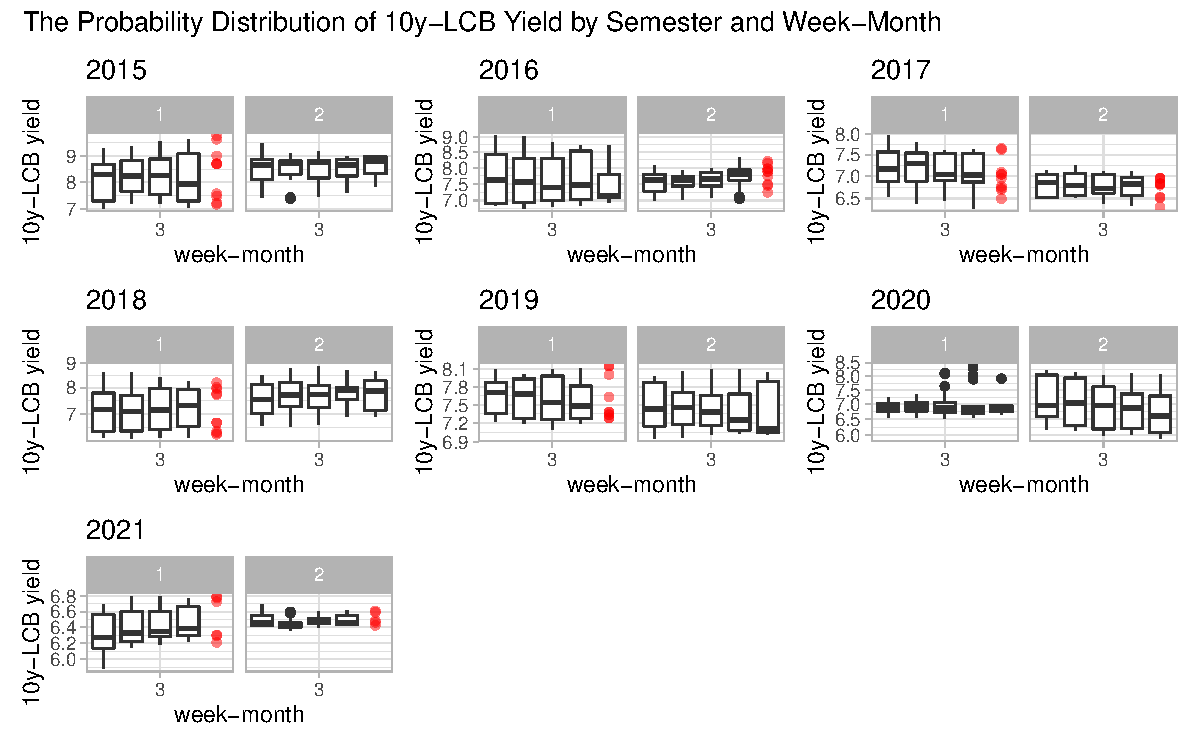
\includegraphics{Untitled_files/figure-latex/unnamed-chunk-3-1.pdf}

Furthermore, as yield is associated with risks, we will group our explanatory variables based on several relevant risk categories.

\hypertarget{external-risk}{%
\subsection{External Risk}\label{external-risk}}

\hypertarget{year-us-treasury-yield}{%
\subsubsection{10-year US Treasury Yield}\label{year-us-treasury-yield}}

The United States of America government's bonds (UST bonds) is generally used as a benchmark for other countries' sovereign bonds. The bonds is considered as the safest instrument hence issuers from other countries will give extra premium over the UST bonds yield in order to compensate additional risks taken by investors for purchasing non-UST bonds.
The UST yield data used in this study is sourced from Bloomberg with the same ticker code ``GRR'' for the 10-year maturity government bonds of the United State of America.

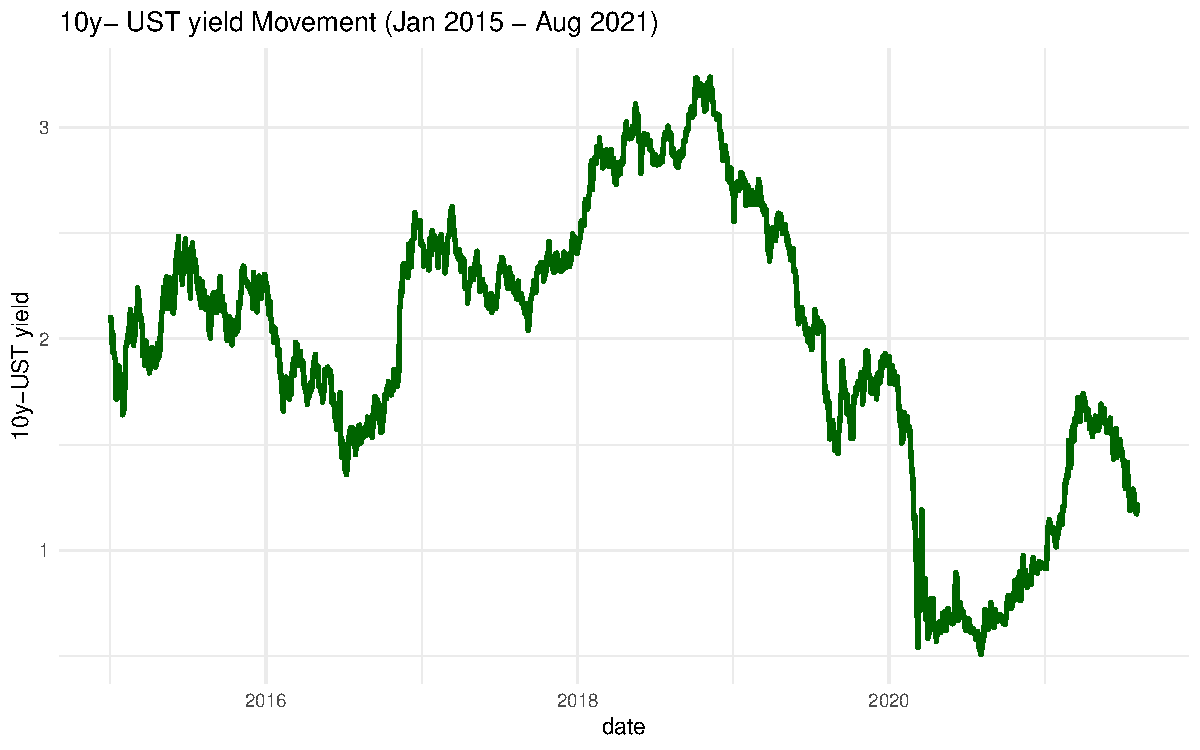
\includegraphics{Untitled_files/figure-latex/unnamed-chunk-5-1.pdf}

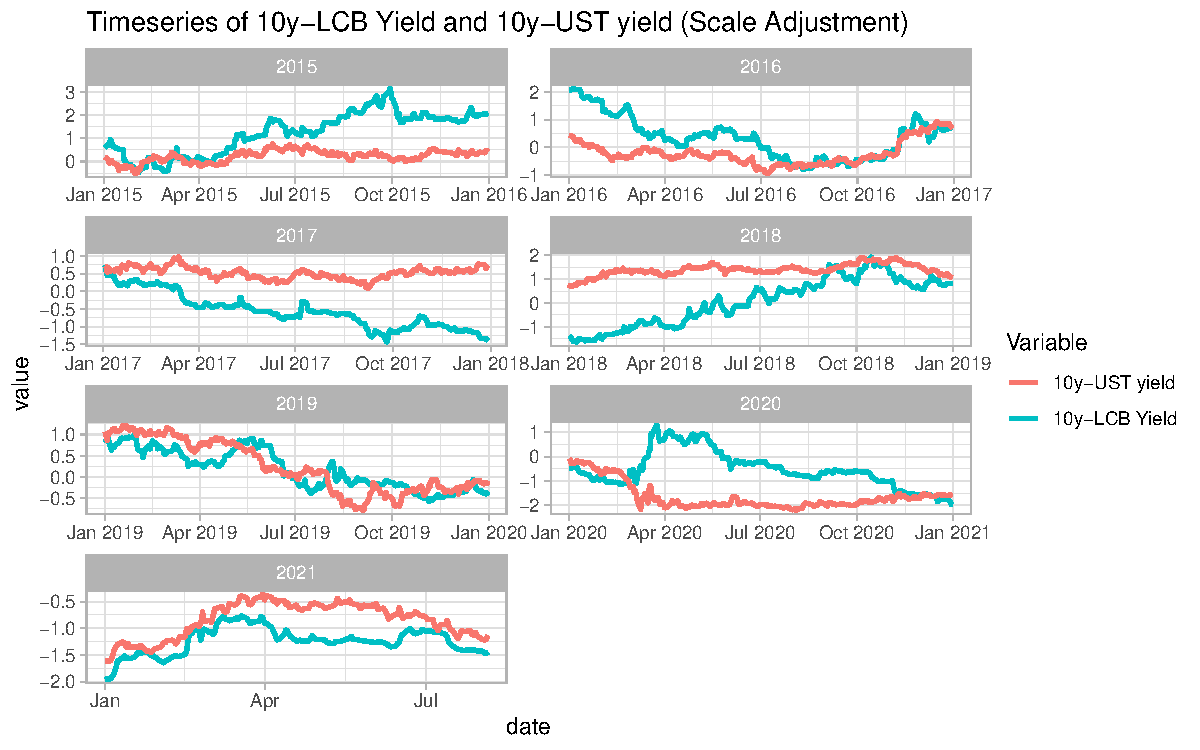
\includegraphics{Untitled_files/figure-latex/unnamed-chunk-6-1.pdf}

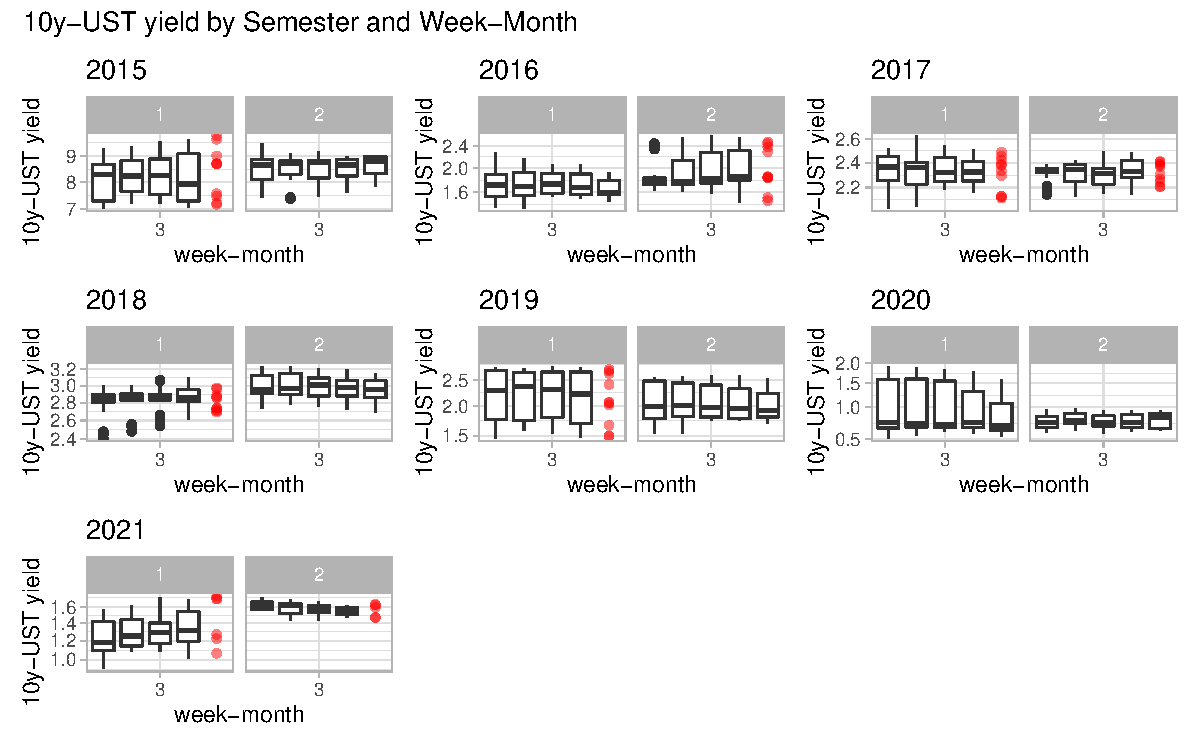
\includegraphics{Untitled_files/figure-latex/unnamed-chunk-7-1.pdf}

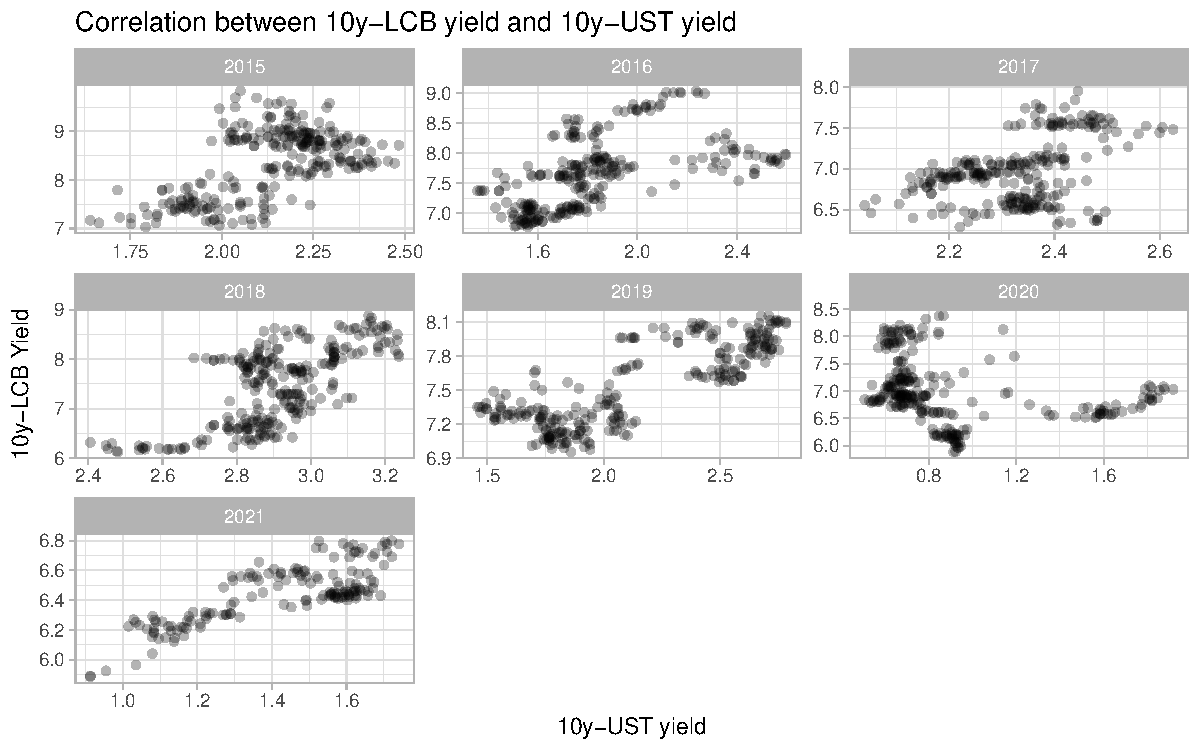
\includegraphics{Untitled_files/figure-latex/unnamed-chunk-8-1.pdf}

\hypertarget{foreign-ownership}{%
\subsubsection{Foreign Ownership}\label{foreign-ownership}}

As per 29 July 2021, foreign investors are holding IDR965 Trillions or 22.5\% of total bonds ownership.

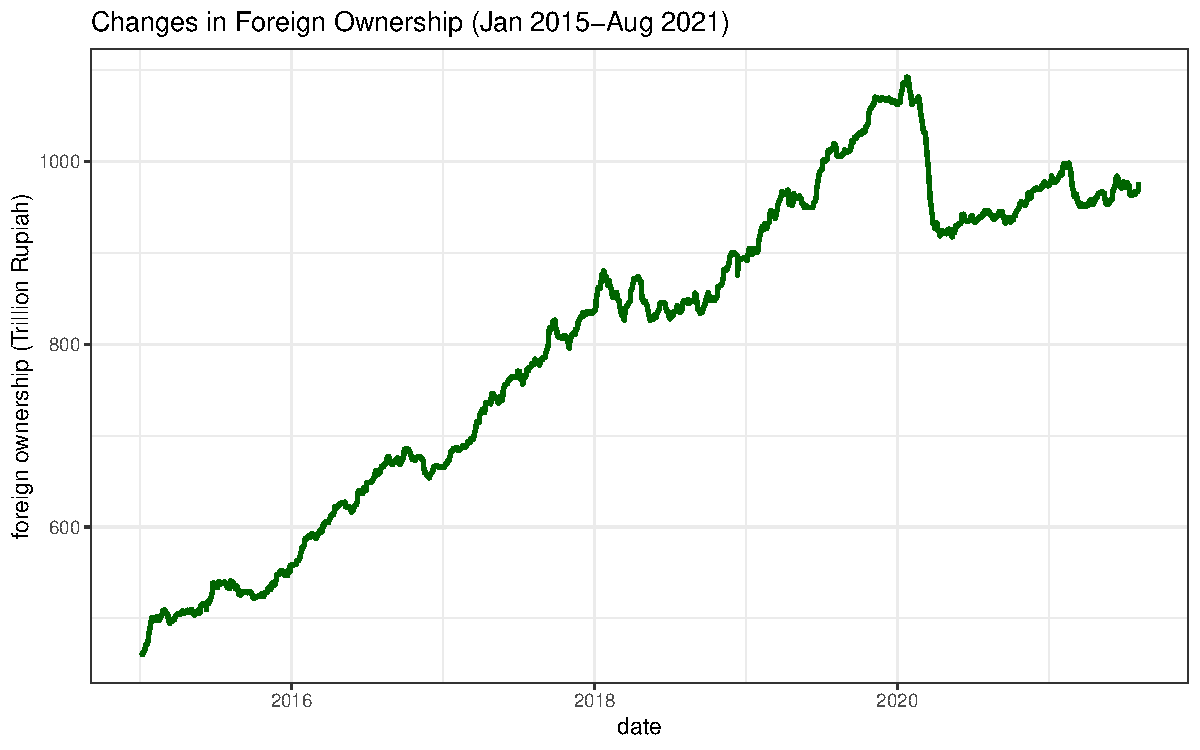
\includegraphics{Untitled_files/figure-latex/unnamed-chunk-10-1.pdf}

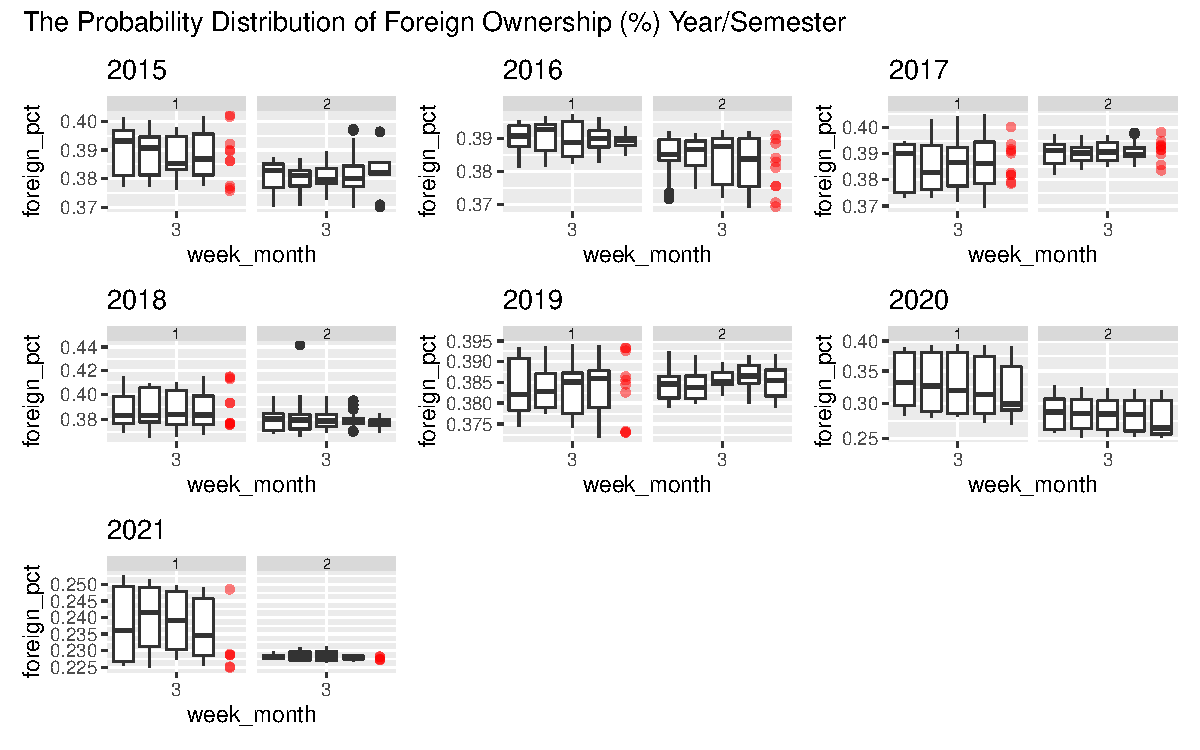
\includegraphics{Untitled_files/figure-latex/unnamed-chunk-11-1.pdf}

The foreign investor's share in the government bonds (including the 10y-LCB) has been reduced dramatically since 2020 due to an increase in both central bank and conventional bank's holdings in the LCB, as shown in figure \ref{fig:ownprop}. The figure shows daily changes in the LCB ownership, grouped by several industries from Jan 2018 until early August of 2021 (data before 2018 is not shown in the plot since it has different classification names for the industries).

\begin{verbatim}
## Warning: Ignoring unknown aesthetics: fill
\end{verbatim}

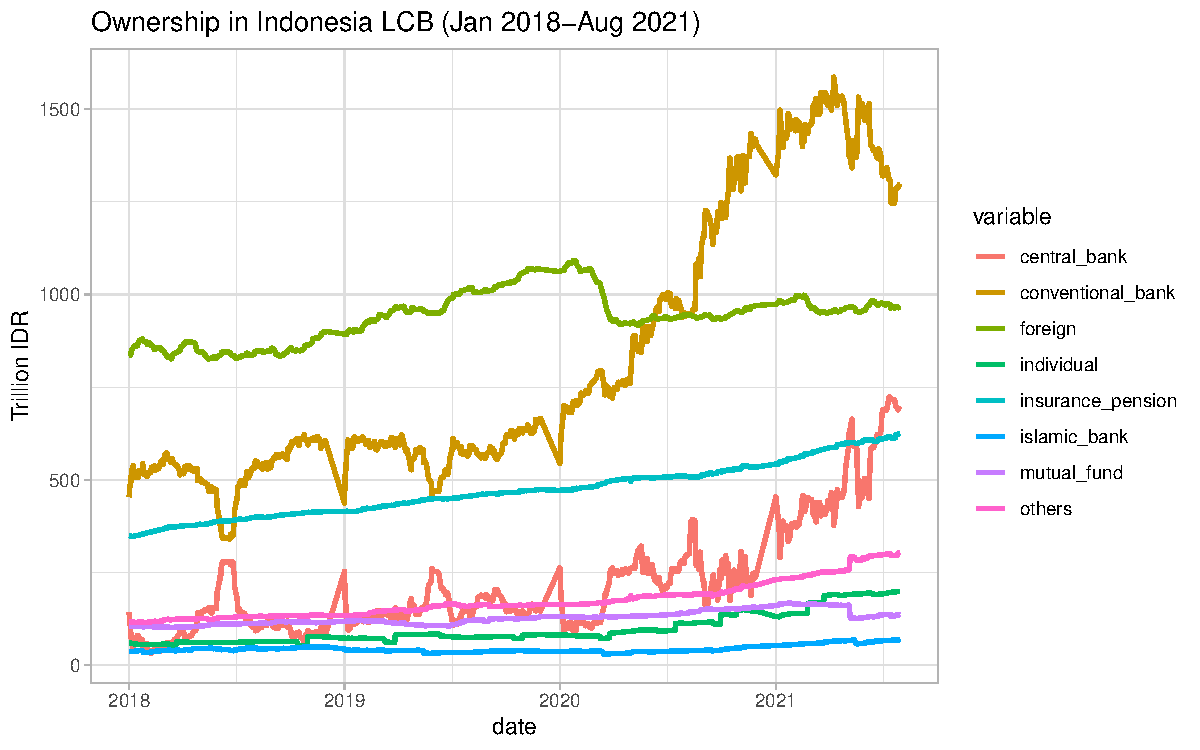
\includegraphics{Untitled_files/figure-latex/ownprop-1.pdf}
In 2020, the central bank seems to move aggressively in purchasing the government bonds through Quantitative Easing (QE) program in order to absorb larger issuance of the bonds which aimed to support large financing for covid19 pandemic. The monetary authority also introduced mandatory purchase regulation for the conventional banks to buy some minimum amount of the bonds, thus the ownership of the banks were also growing large and beyond the foreigner's ownership.

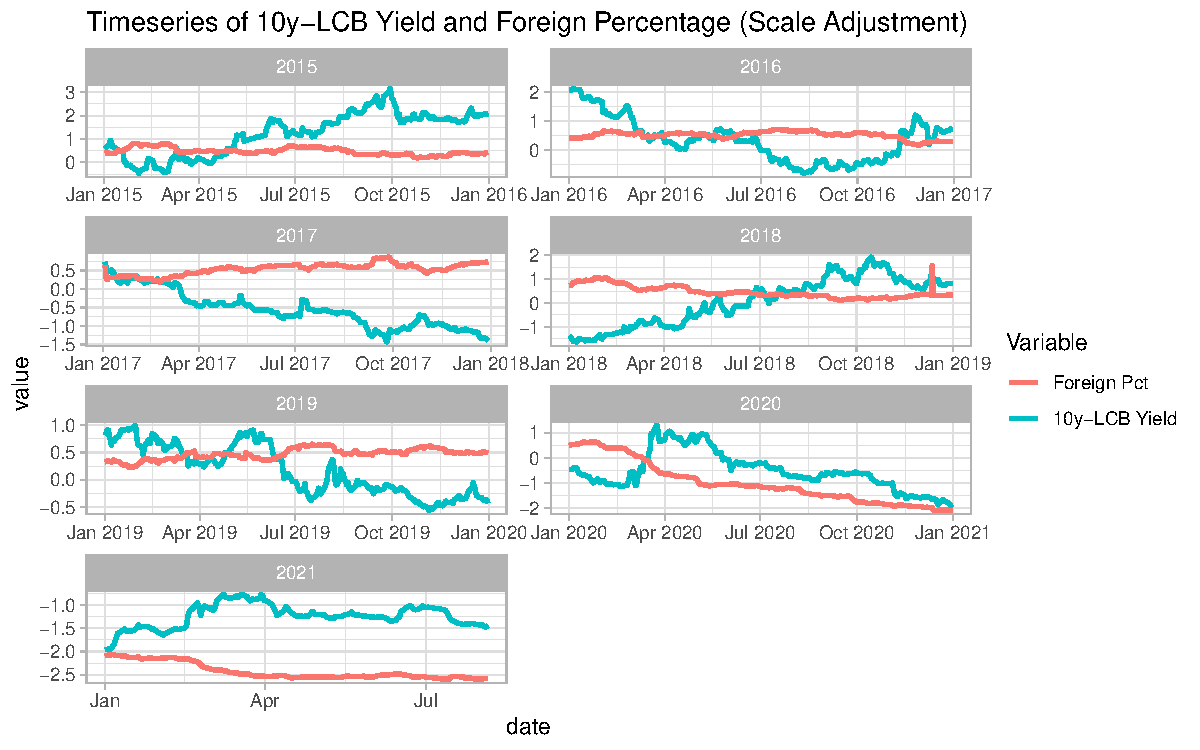
\includegraphics{Untitled_files/figure-latex/unnamed-chunk-12-1.pdf}

The yearly correlation between the foreign ownership and the 10y-LCB yield can be seen in figure \ref{fig:corfor}. In general, the plot shows negative correlation between these two variables, except for 2020 in which foreigner's dominant holding of the LCB was mainly reduced by the increase of conventional banks and the central bank's holdings. Thus, despite a decrease in the foreigner's portion, the yield was kept lowered since the banks and the central bank increased their holdings.

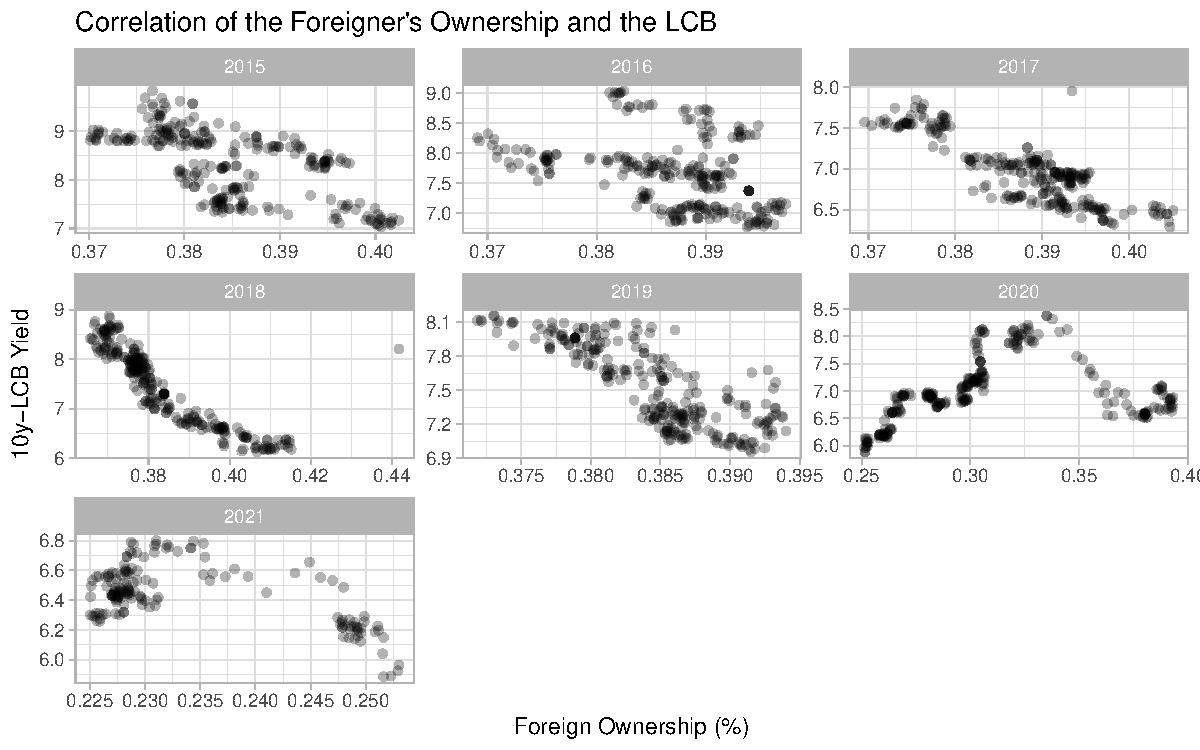
\includegraphics{Untitled_files/figure-latex/corfor-1.pdf}

\hypertarget{default-risk-5-year-credit-default-swap}{%
\subsection{Default Risk (5-year Credit Default Swap)}\label{default-risk-5-year-credit-default-swap}}

A credit default swap (CDS) is a derivative contract that allows investors to hedge against the default of a borrower. This provides a market-based measure of the credit-risk premium. As mentioned by \textcite{codogno}, CDS spreads can be seen as indication of the perceived credit risk by investors. This study uses data of Indonesia's 5y-CDS which is gathered from Bloomberg platform for period of Jan 2015-August 2021.

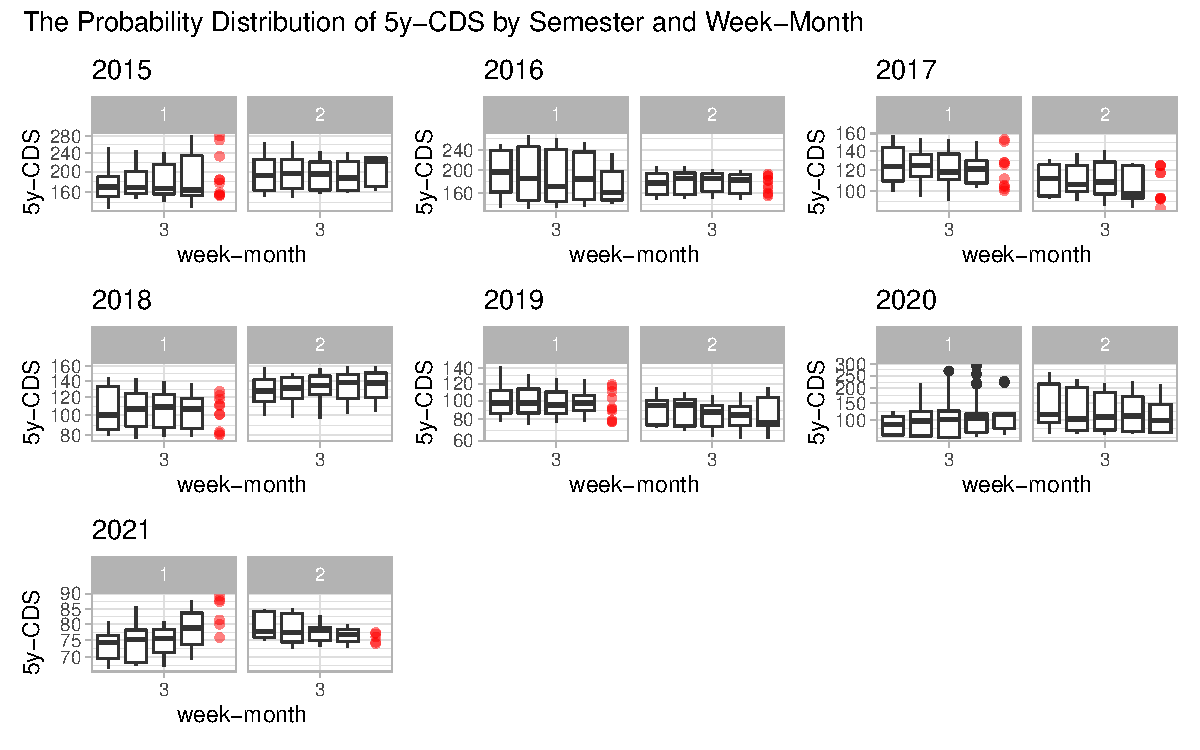
\includegraphics{Untitled_files/figure-latex/cds-1.pdf}

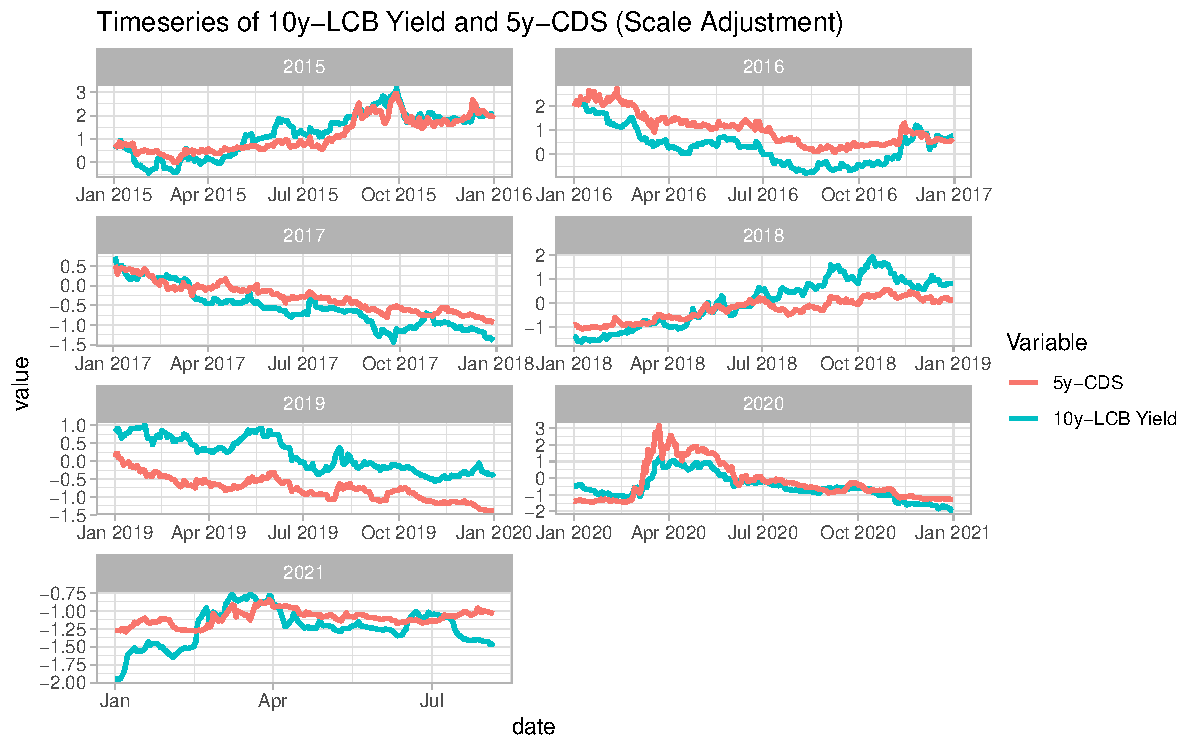
\includegraphics{Untitled_files/figure-latex/unnamed-chunk-13-1.pdf}

The yearly correlation between the CDS and the yield is shown in figure \ref{fig:corcds}. The plot shows strong relationship between the two variables in all observed years.

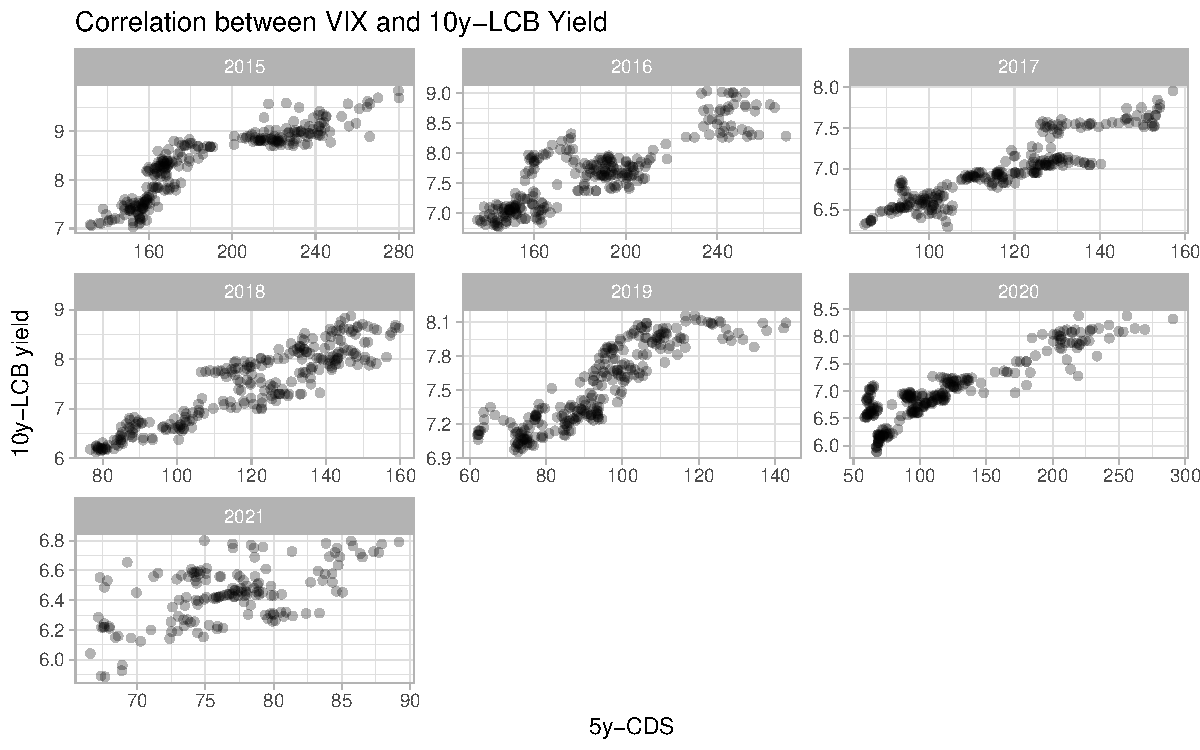
\includegraphics{Untitled_files/figure-latex/corcds-1.pdf}

\hypertarget{financial-market-risk-volatility-index}{%
\subsection{Financial Market Risk (Volatility Index)}\label{financial-market-risk-volatility-index}}

Volatility Index which is a shorter term for Chicago Board Options Exchange's (CBOE) Volatility Index was first introduced by the CBOE to measure the relative strength of short-term price changes of the S\&P 500 index (SPX) in real-time. One of the main purposes of the VIX Index as suggested by Whaley \autocite*{Whaley2009} is it can be used to quantify expected short-term volatility and to track historical volatility using index option prices.

Beyond the USA, the VIX Index is also commonly used in other countries to quantify the volatility of stock markets. Data of Indonesia's VIX Index used in this study is generated from Bloomberg platform.

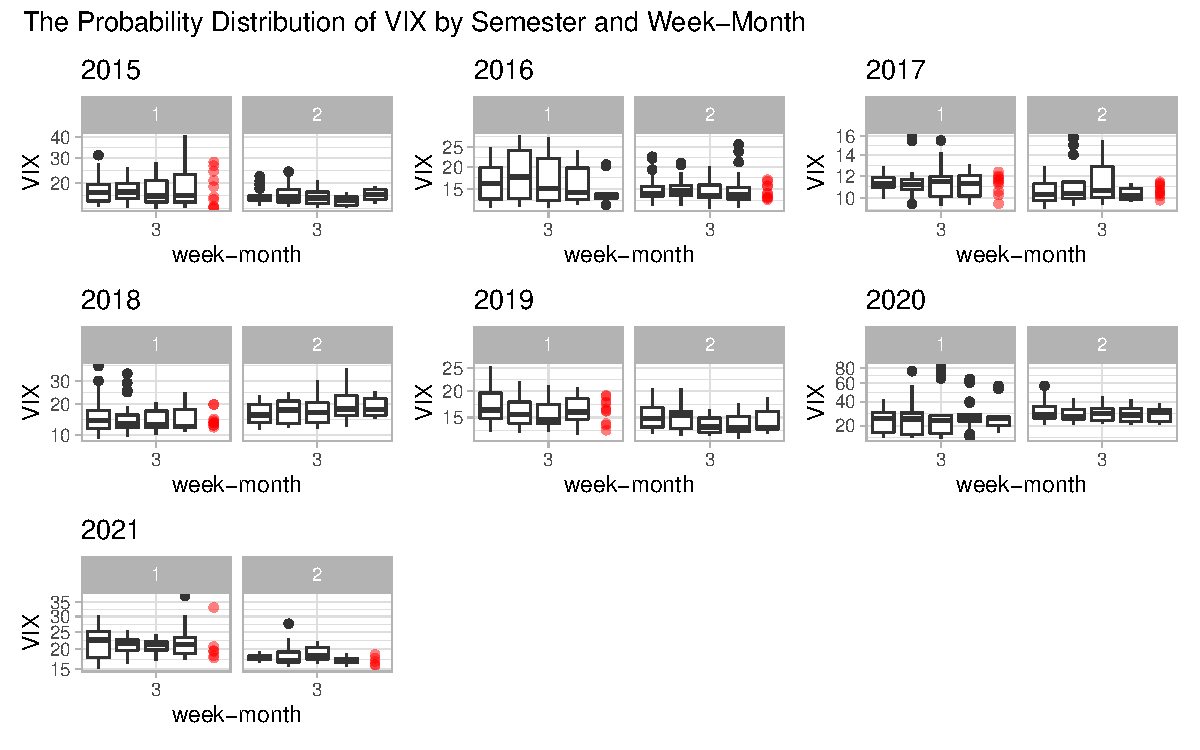
\includegraphics{Untitled_files/figure-latex/unnamed-chunk-14-1.pdf}

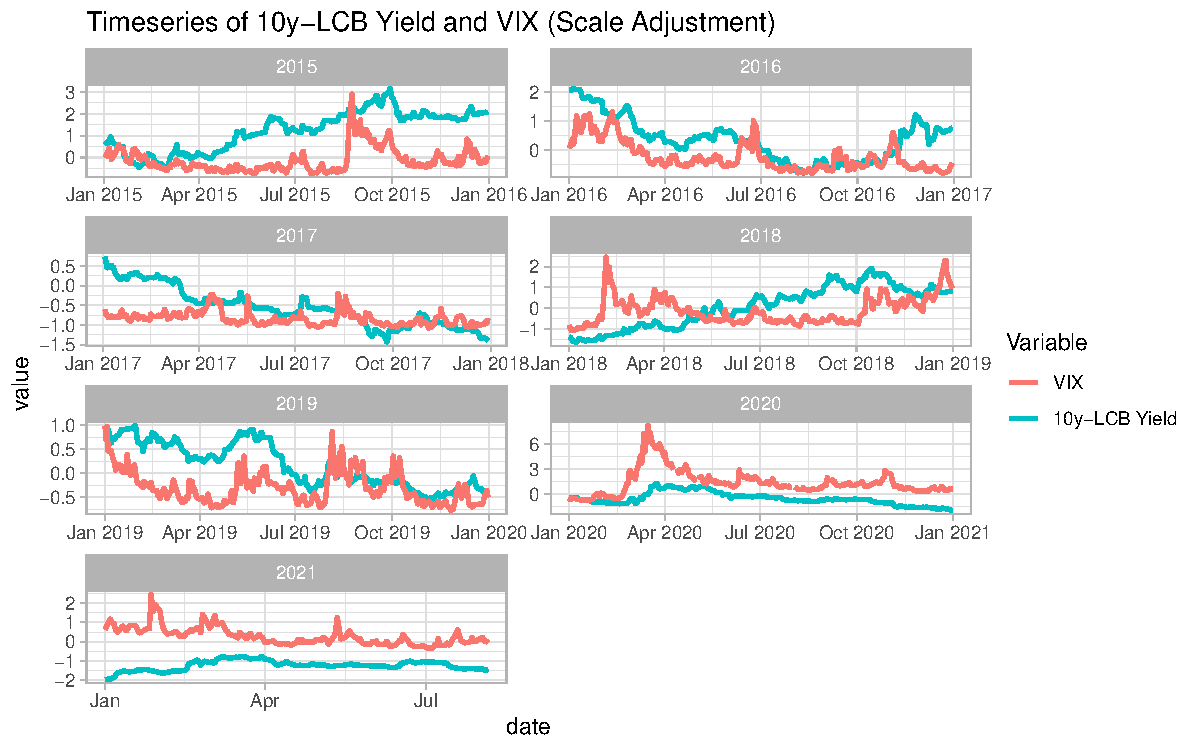
\includegraphics{Untitled_files/figure-latex/unnamed-chunk-15-1.pdf}

The yearly correlation between the VIX and the yield is shown in figure \ref{fig:corvix}. The plot shows a \textbf{non-linear relationship} between the two variables in all observed years. Thus, we will introduce a quadratic term to the VIX variable to handle this issue in our linear model.

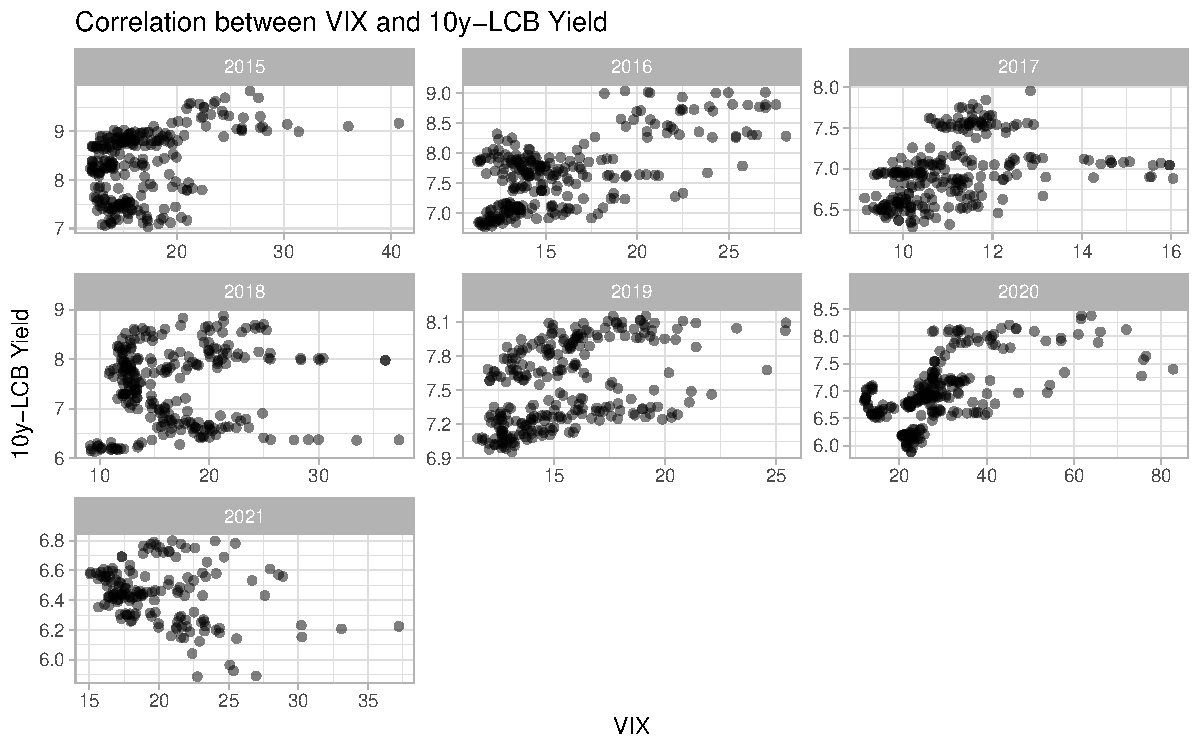
\includegraphics{Untitled_files/figure-latex/corvix-1.pdf}

\hypertarget{macroeconomic-risk-exchange-rate-usdidr}{%
\subsection{Macroeconomic Risk (Exchange Rate USD/IDR)}\label{macroeconomic-risk-exchange-rate-usdidr}}

The data for foreign exchange (fx) rate of USD against Rupiah is using middle rate, calculated from Bank Indonesia's buy and sell fx rates of each working day \footnote{The foreign exchange data can be downloaded at \url{https://www.bi.go.id/en/statistik/informasi-kurs/transaksi-bi/Default.aspx}}. For non-working days, data is imputed from the rate of a previous working day.

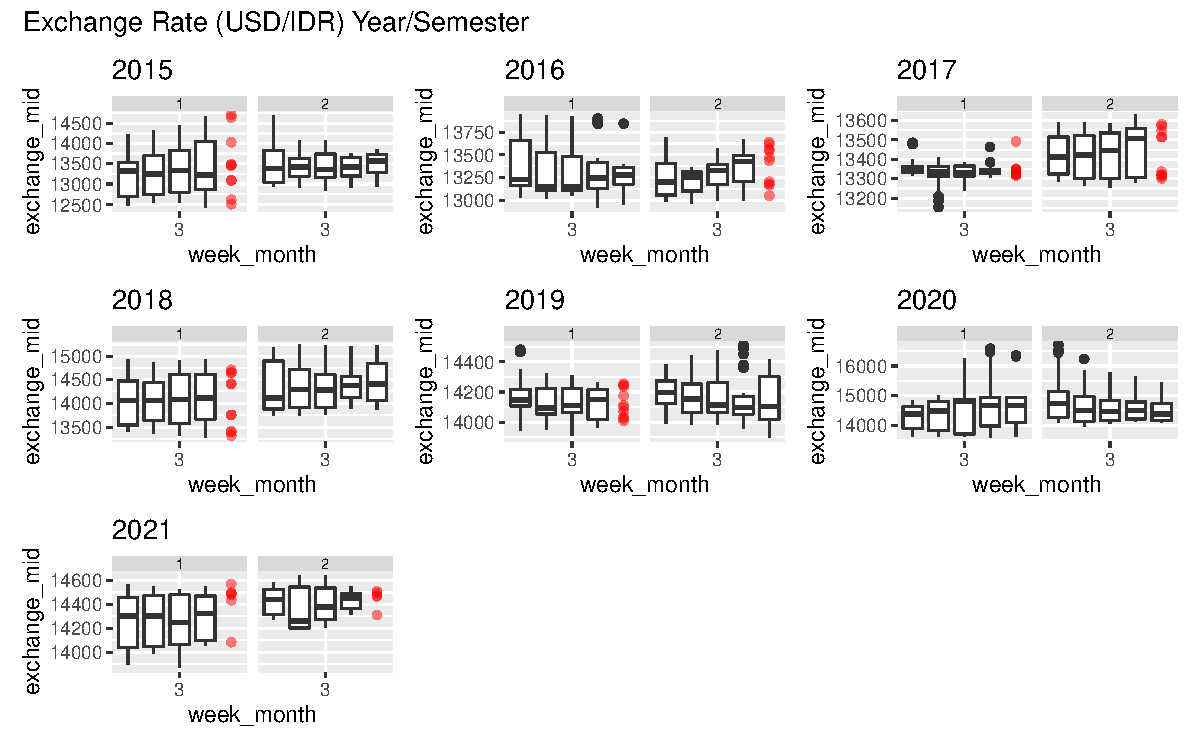
\includegraphics{Untitled_files/figure-latex/unnamed-chunk-16-1.pdf}

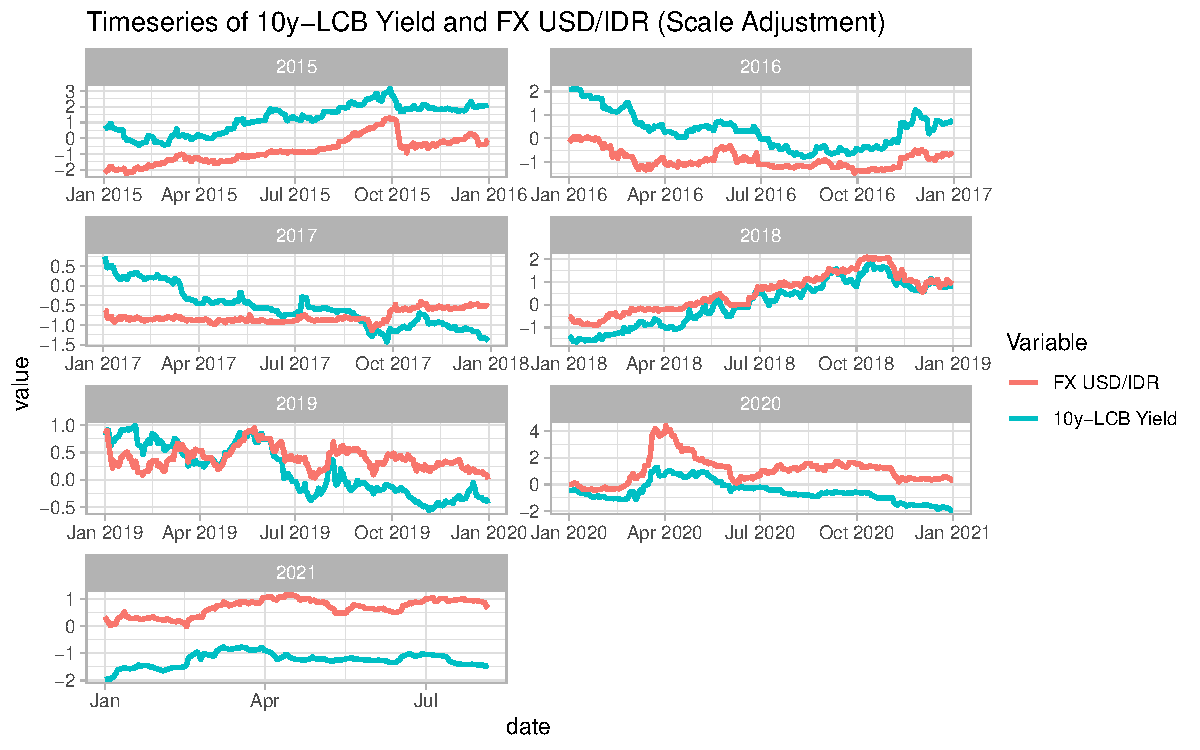
\includegraphics{Untitled_files/figure-latex/unnamed-chunk-17-1.pdf}

The yearly correlation between the exchange rate and the yield is shown in figure \ref{fig:corfx}. The plot shows a strong positive relationship between the two variables in all observed years, except for 2017 which has a quite different pattern.

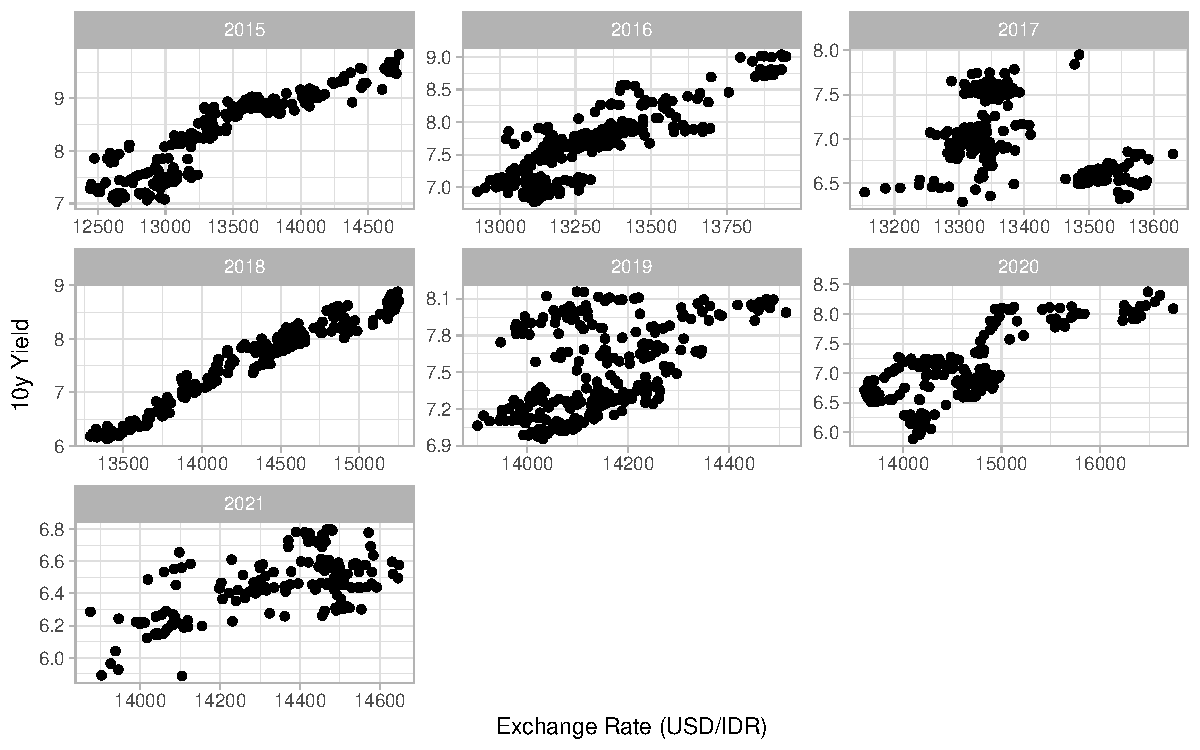
\includegraphics{Untitled_files/figure-latex/corfx-1.pdf}

\hypertarget{system-risk-primary-dealers-behavior}{%
\subsection{System Risk (Primary Dealers Behavior)}\label{system-risk-primary-dealers-behavior}}

Primary dealers system in Indonesia has been established since 2007. The system is expected to run several functions as shown in more developed economies. Arnone and Arden \autocite*{Arnone2003} describe role of primary dealers as intermediary between debt managers and investors in primary market, bookmakers and bonds distributors, liquidity provider between primary and secondary market, promoter of continuous market and efficient price discovery, and adviser to government.

In 2021, there are 20 primary dealers of conventional bonds comprise of 16 conventional banks and 4 securities companies. For sharia bonds, there are also 20 primary dealers consist of 13 conventional banks, 3 Islamic banks and 4 securities companies. Primary dealers are required to participate in every auction and to bid for a minimum quantity of the total offering amount. They can bid both on behalf of their customers and for their own accounts. As primary dealers can participate in competitive bidding in primary market as well as buy and sell in secondary market, they have direct contribution on forming yield of sovereign bonds.

Tchuindjo \autocite*{Tchuindjo2015} writes that primary dealers will make bilateral contracts for the offered securities as soon as auction announced, known as pre-sale or when-issued market. Mercer et al. \autocite*{Mercer2013} argue that they will be able to ``discover'' the ultimate auction price since in pre-sale period. Many primary dealers are also believed to often short in the when-issued market \autocite{Nyborg2004}, which encourages them to bid aggressively and assign lower prices to the auctioned securities \autocite{Tchuindjo2015}, meaning higher demanded yields.

Thus, our analysis will be based on an assumption that primary dealers' strategic behavior in the auctions can affect sovereign bonds yield. To check this assumption, we use dummy variables of ``auction days'' that representing the pre-sale/when-issued period and ``non-auction days'' that representing regular workdays. Referring to Nyborg et al. \autocite*{Nyborg2004} pre-sale period is described as days started from the day of auction announcement (T-3) until a moment before bonds is distributed on the day of settlement (T+2). For simplicity, we define auction days as days started from T-3 until T+1. Here, we exclude the day of settlement (T+2) since bonds is usually distributed by the Central Bank in the morning of the settlement day. In addition, we only include auction days that offer benchmark series of the 10-year sovereign bonds in the auction day (T). Before 2019, the 10-year series is not regularly offered in the auction.

In the graph below, we will observe the pattern of 10-year yield movement and the dummy categories.

\begin{figure}
\centering
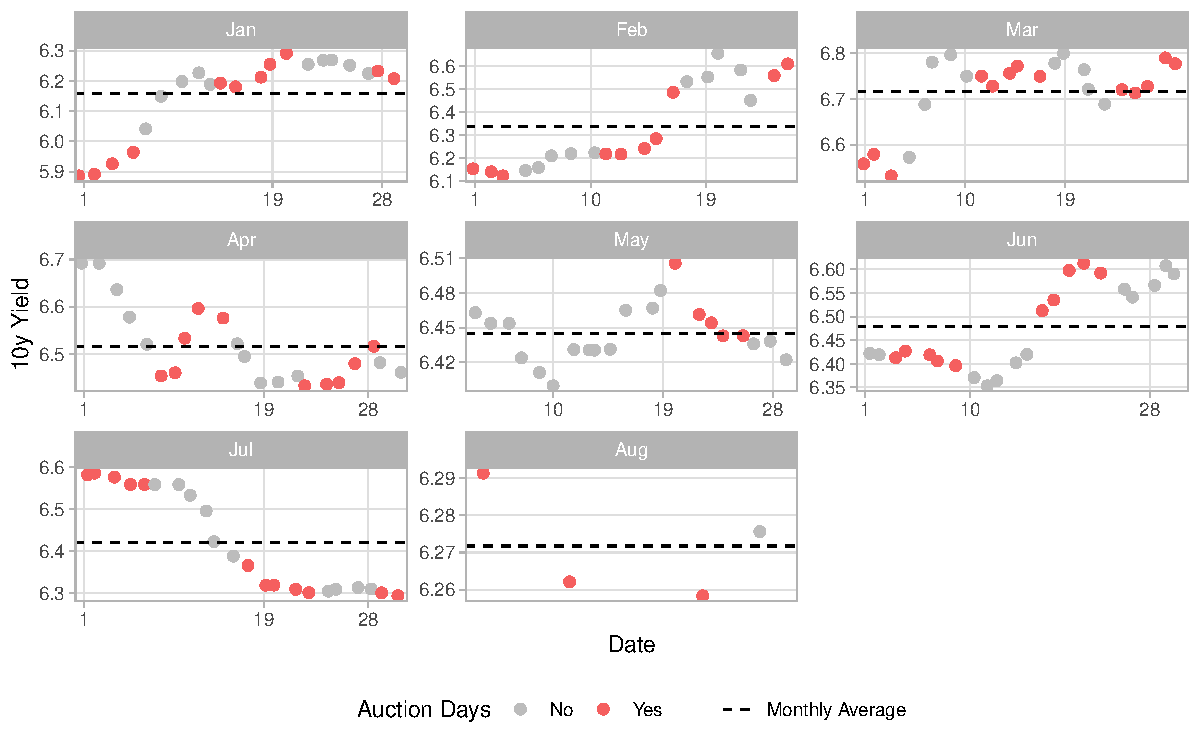
\includegraphics{Untitled_files/figure-latex/yieldmove-1.pdf}
\caption[\label{fig:yieldmove}10-year Yield's Movement during Auction Days during January-August 2021]{\label{fig:yieldmove}10-year Yield's Movement during Auction Days during January-August 2021\footnotemark{}}
\end{figure}
\footnotetext{Full period of observation can be seen in the Appendix}

From figure \ref{fig:yieldmove}, volatility in non auction days (post auction) is also tend to be higher than volatility in auction days.

\begin{figure}
\centering
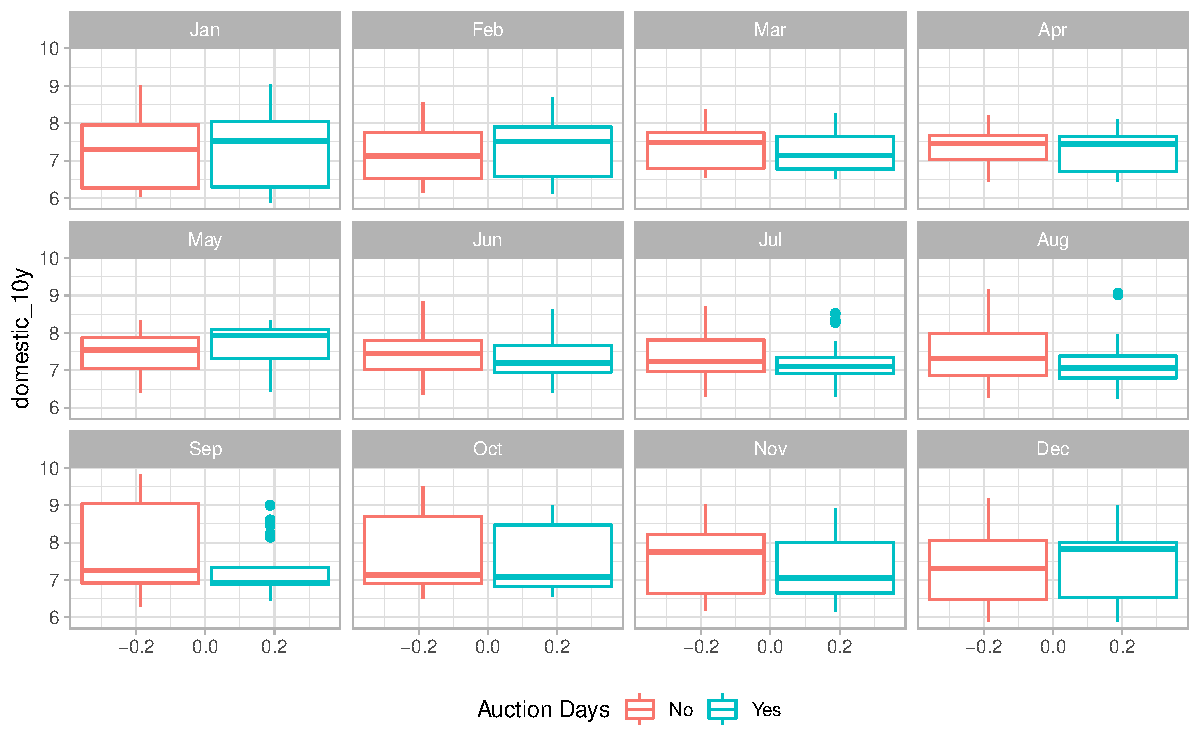
\includegraphics{Untitled_files/figure-latex/unnamed-chunk-18-1.pdf}
\caption{\label{fig:unnamed-chunk-18}10-year Yield's Movement during Auction Days from 2016-2021}
\end{figure}

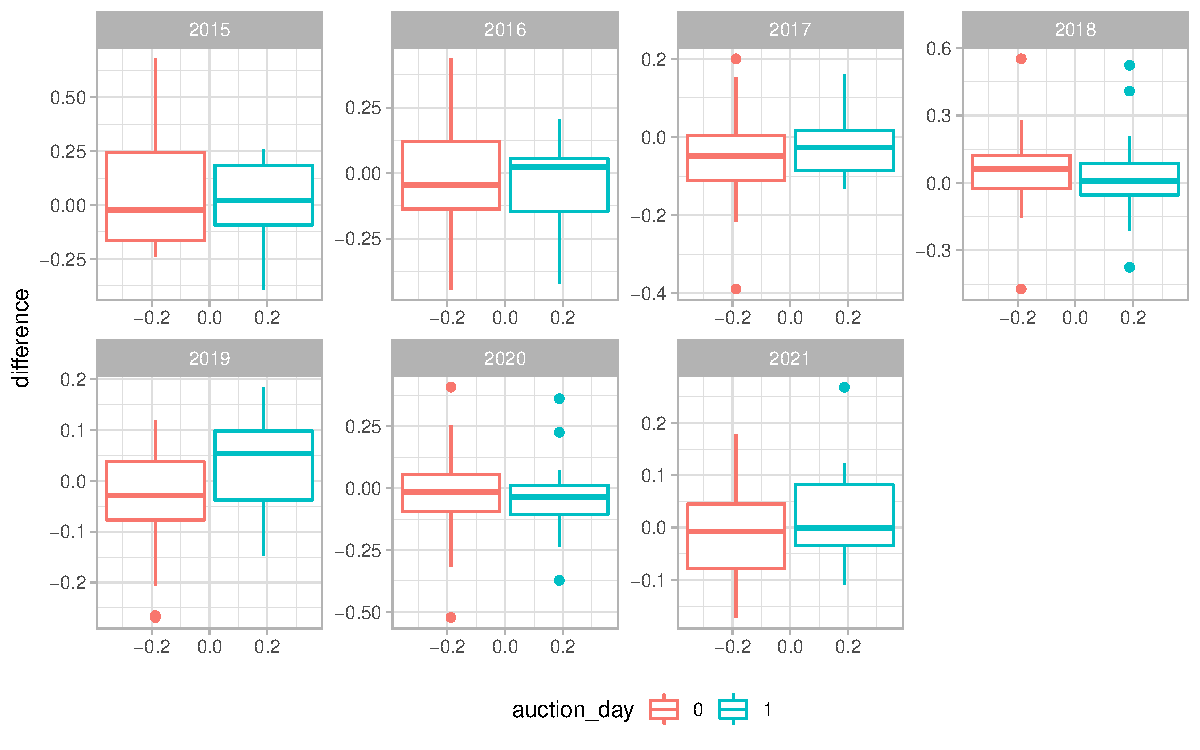
\includegraphics{Untitled_files/figure-latex/unnamed-chunk-20-1.pdf}

We analyze the difference in yield's movement between auction days and non-auction days. The difference is calculated by subtracting yield of the last and first days in each period. The summary table of the yield difference (showing first 10 rows) can be seen in table \ref{tab:yielddiftable}.

\begin{table}[H]
\centering
\begin{tabular}{r|l|l|r|r|r}
\hline
auction\_day & date\_from & date\_to & domestic\_10y\_from & domestic\_10y\_to & difference\\
\hline
1 & 2015-01-02 & 2015-01-07 & 7.859 & 8.117 & 0.258\\
\hline
0 & 2015-01-08 & 2015-01-14 & 8.066 & 7.828 & -0.238\\
\hline
1 & 2015-01-15 & 2015-01-21 & 7.791 & 7.401 & -0.390\\
\hline
0 & 2015-01-22 & 2015-02-10 & 7.370 & 7.195 & -0.175\\
\hline
1 & 2015-02-11 & 2015-02-17 & 7.412 & 7.393 & -0.019\\
\hline
0 & 2015-02-18 & 2015-02-25 & 7.195 & 7.142 & -0.053\\
\hline
1 & 2015-02-26 & 2015-03-04 & 7.104 & 7.289 & 0.185\\
\hline
0 & 2015-03-05 & 2015-03-25 & 7.404 & 7.336 & -0.068\\
\hline
1 & 2015-03-26 & 2015-04-01 & 7.378 & 7.519 & 0.141\\
\hline
0 & 2015-04-02 & 2015-05-05 & 7.507 & 8.084 & 0.577\\
\hline
\end{tabular}
\end{table}

\begin{verbatim}
## Warning: `as_data_frame()` was deprecated in tibble 2.0.0.
## Please use `as_tibble()` instead.
## The signature and semantics have changed, see `?as_tibble`.
## This warning is displayed once every 8 hours.
## Call `lifecycle::last_warnings()` to see where this warning was generated.
\end{verbatim}

\begin{verbatim}
## Warning: Removed 1 row(s) containing missing values (geom_path).
\end{verbatim}

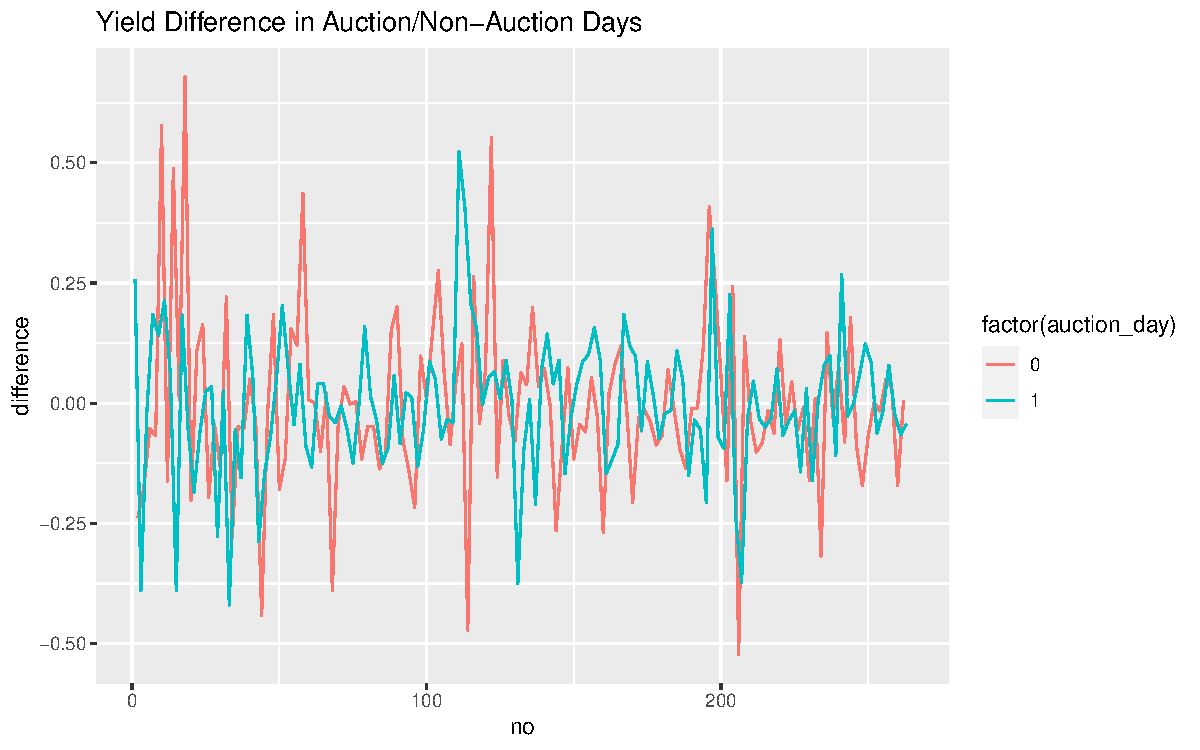
\includegraphics{Untitled_files/figure-latex/yielddif_line-1.pdf}

\begin{verbatim}
## Warning: Removed 1 row(s) containing missing values (geom_path).
\end{verbatim}

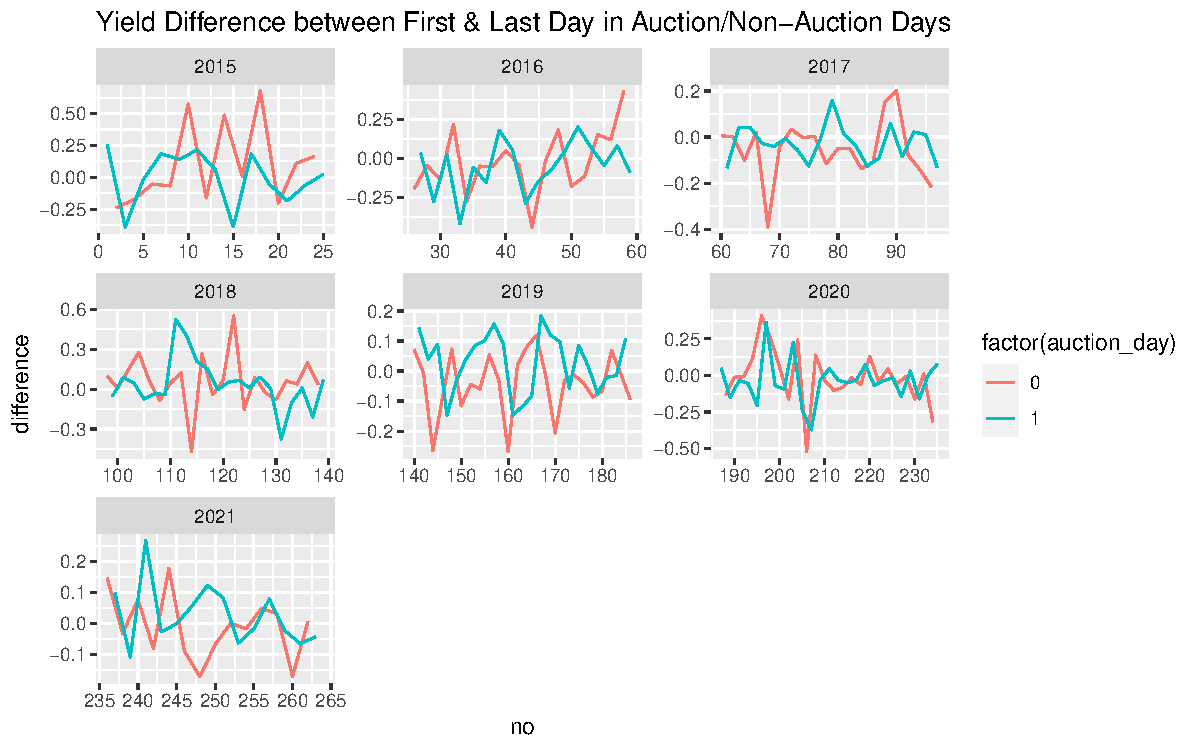
\includegraphics{Untitled_files/figure-latex/yielddif_line-2.pdf}

\begin{figure}
\centering
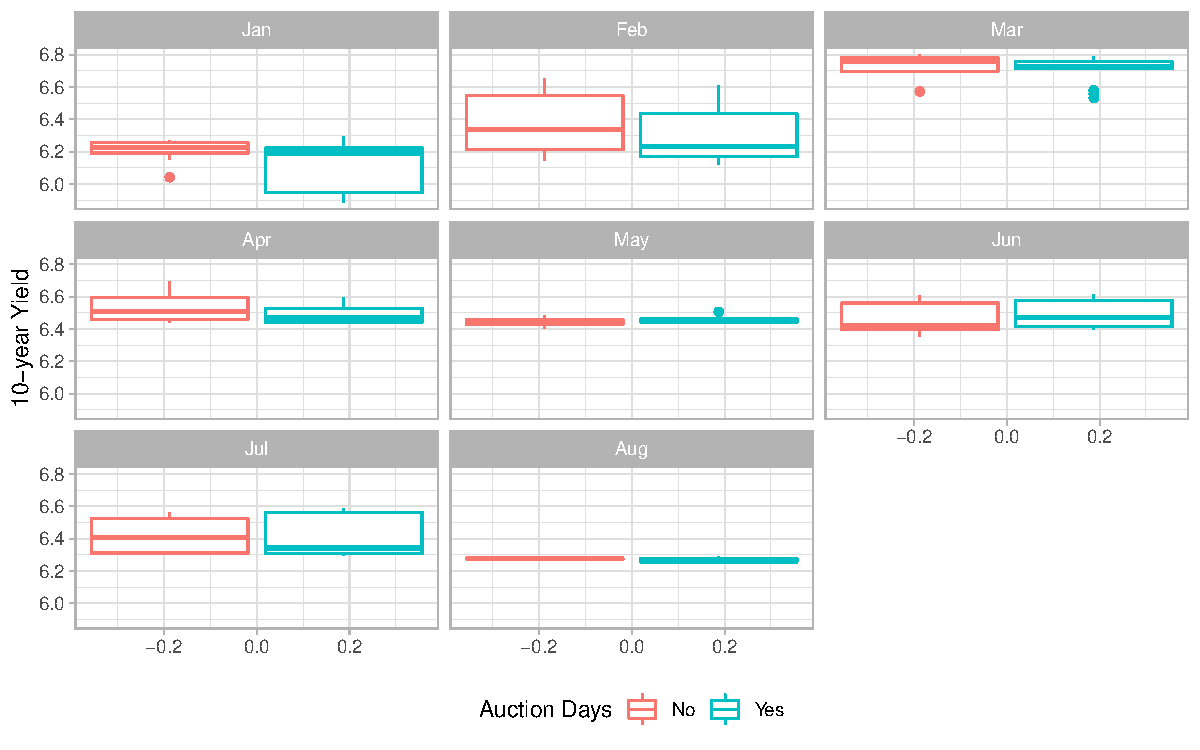
\includegraphics{Untitled_files/figure-latex/unnamed-chunk-21-1.pdf}
\caption[\label{fig:unnamed-chunk-21}Boxplot of 10-year Yield's Movement during Auction Days during January-August 2021]{\label{fig:unnamed-chunk-21}Boxplot of 10-year Yield's Movement during Auction Days during January-August 2021\footnotemark{}}
\end{figure}
\footnotetext{ibid}

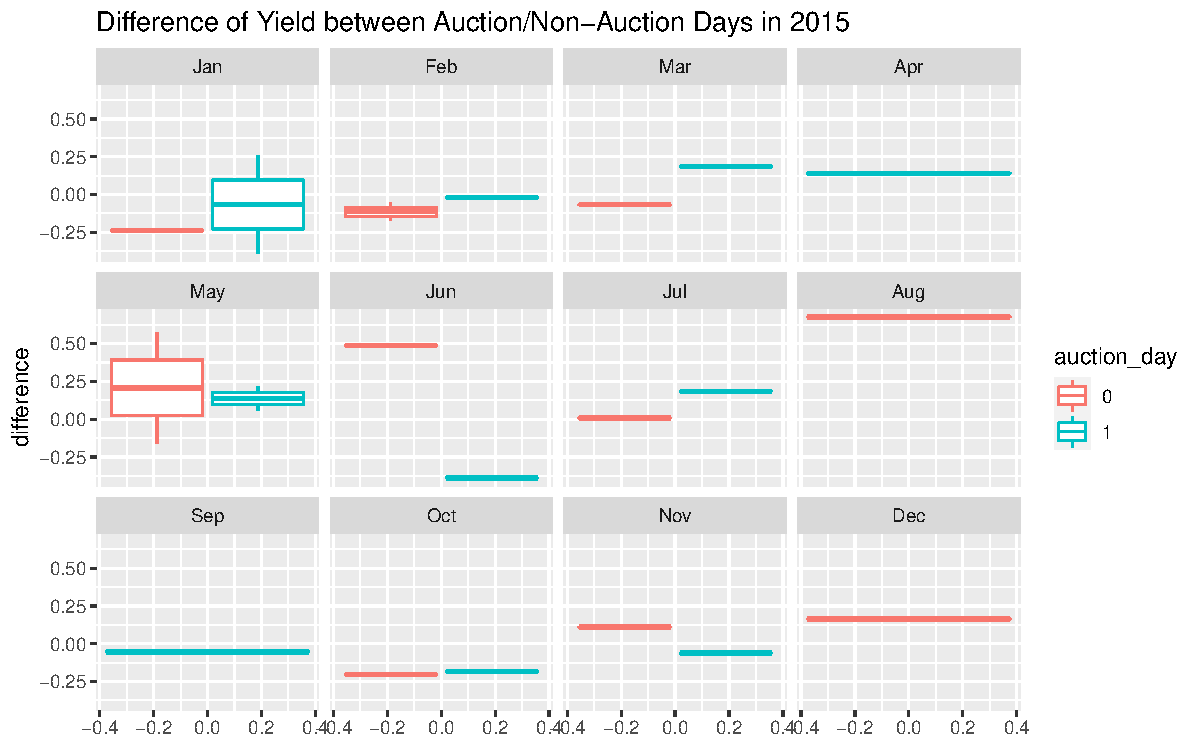
\includegraphics{Untitled_files/figure-latex/unnamed-chunk-22-1.pdf} 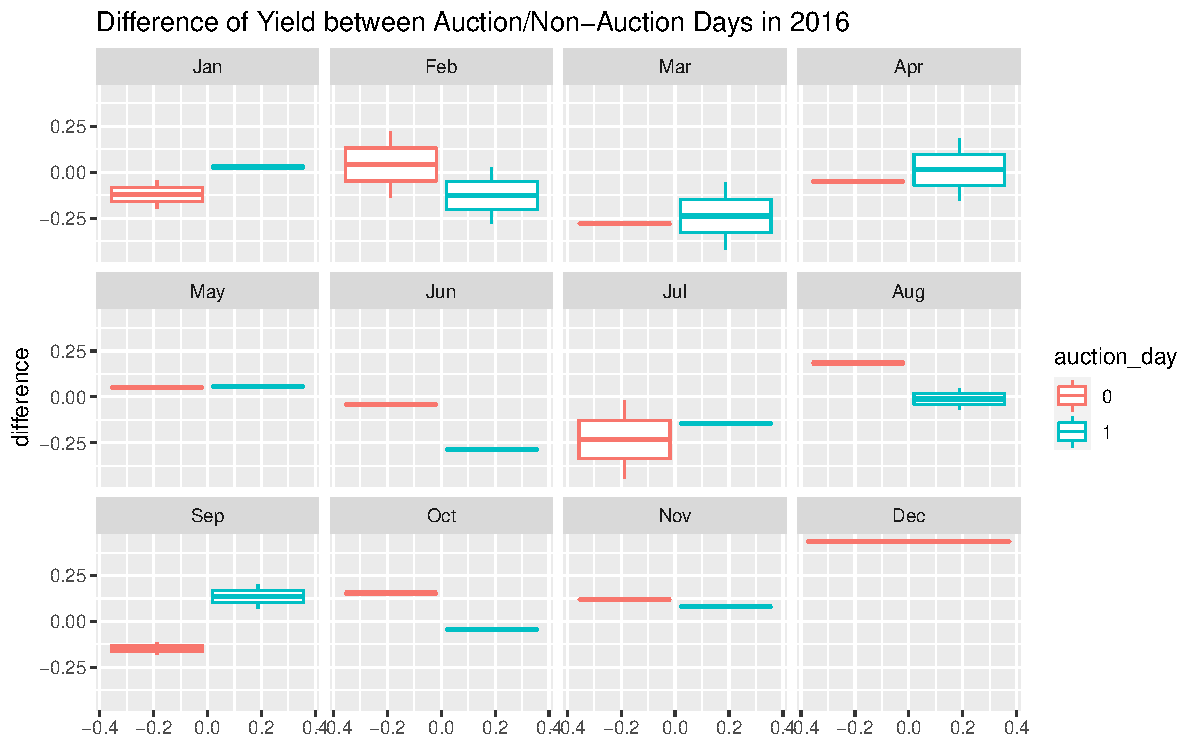
\includegraphics{Untitled_files/figure-latex/unnamed-chunk-22-2.pdf} 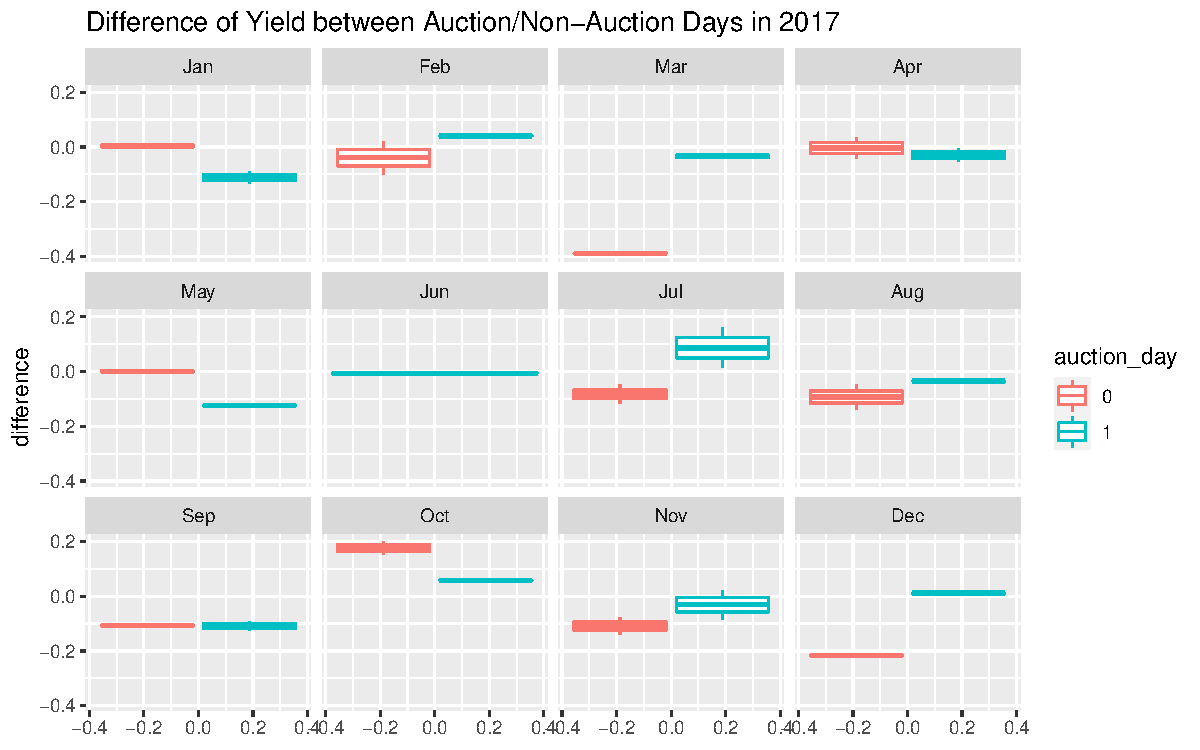
\includegraphics{Untitled_files/figure-latex/unnamed-chunk-22-3.pdf} 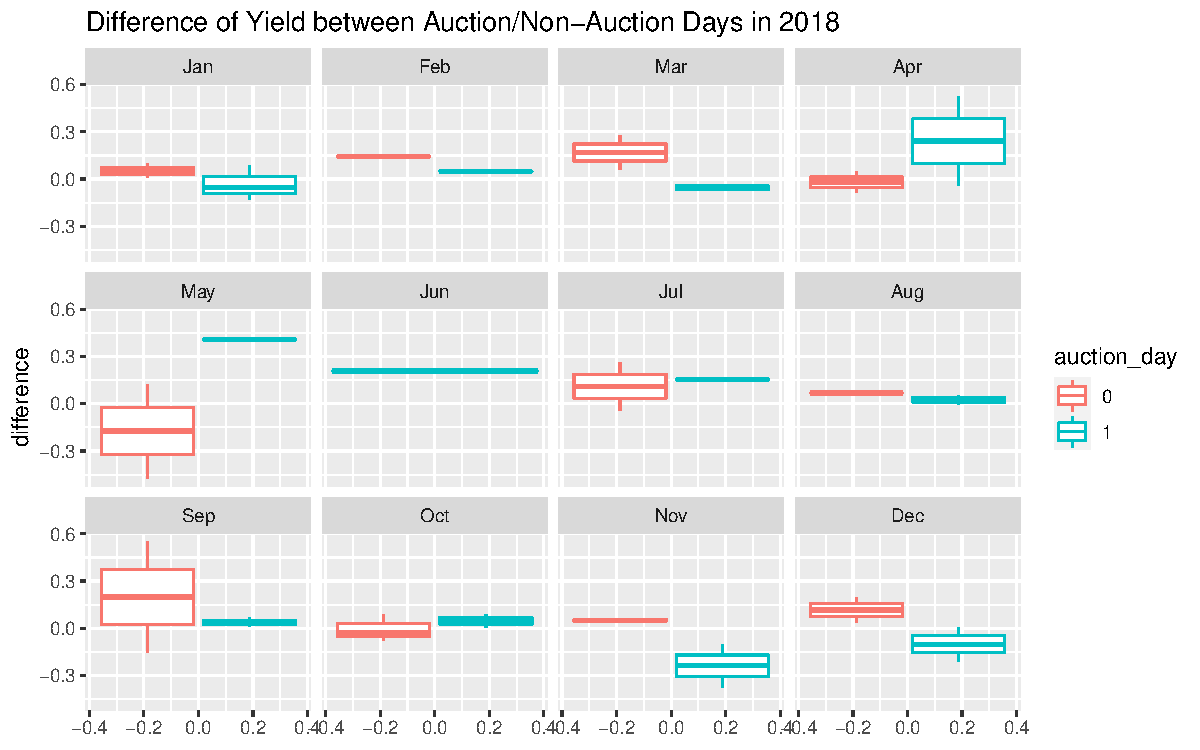
\includegraphics{Untitled_files/figure-latex/unnamed-chunk-22-4.pdf}

\newpage

\hypertarget{research-methodology}{%
\section{Research Methodology}\label{research-methodology}}

\hypertarget{stationary-test}{%
\subsection{Stationary Test}\label{stationary-test}}

To ensure that our model is not biased, we will conduct stationery test on the variables using Augmented Dicky Fuller (ADF) and KPSS.

\hypertarget{cointegration-test}{%
\subsection{Cointegration test}\label{cointegration-test}}

\hypertarget{visual-test}{%
\subsubsection{Visual Test}\label{visual-test}}

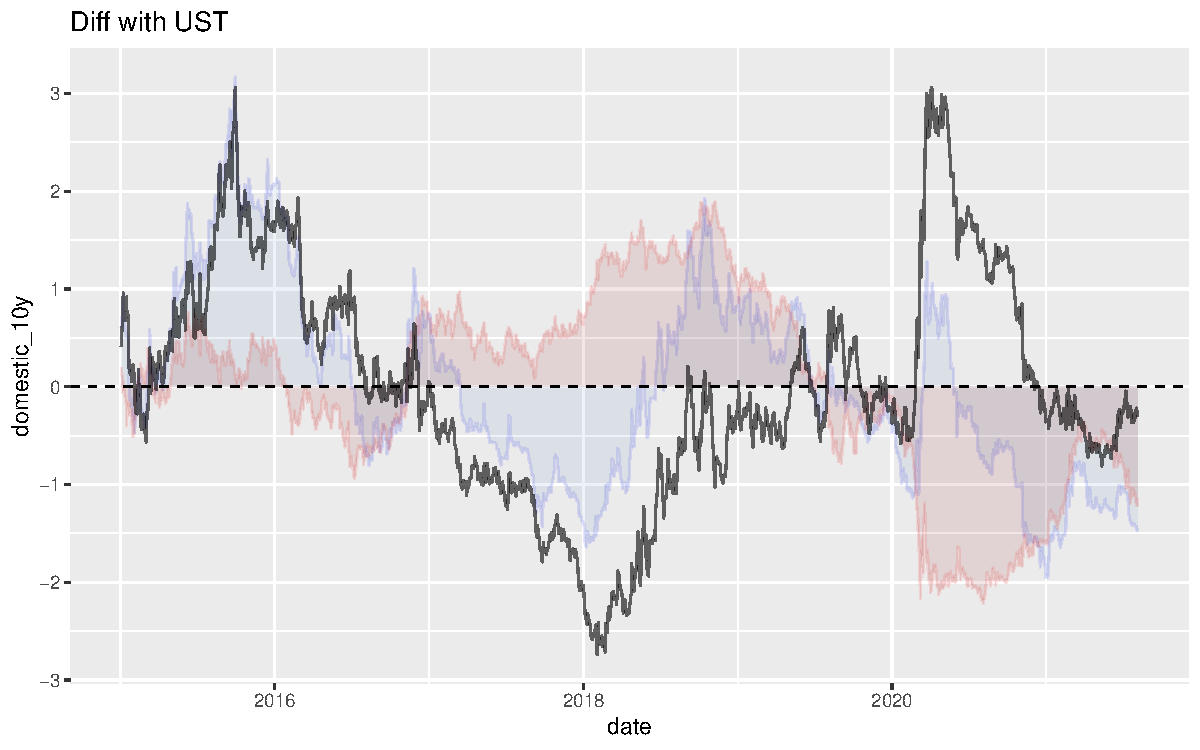
\includegraphics{Untitled_files/figure-latex/unnamed-chunk-24-1.pdf} 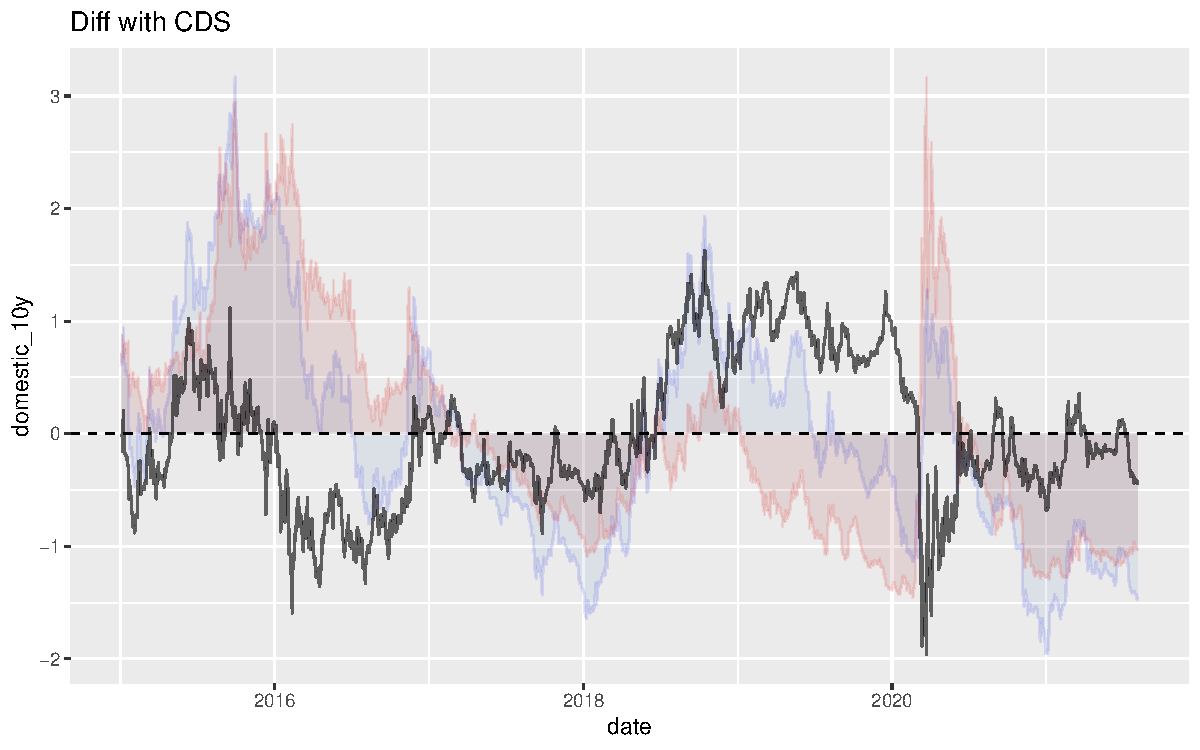
\includegraphics{Untitled_files/figure-latex/unnamed-chunk-24-2.pdf} 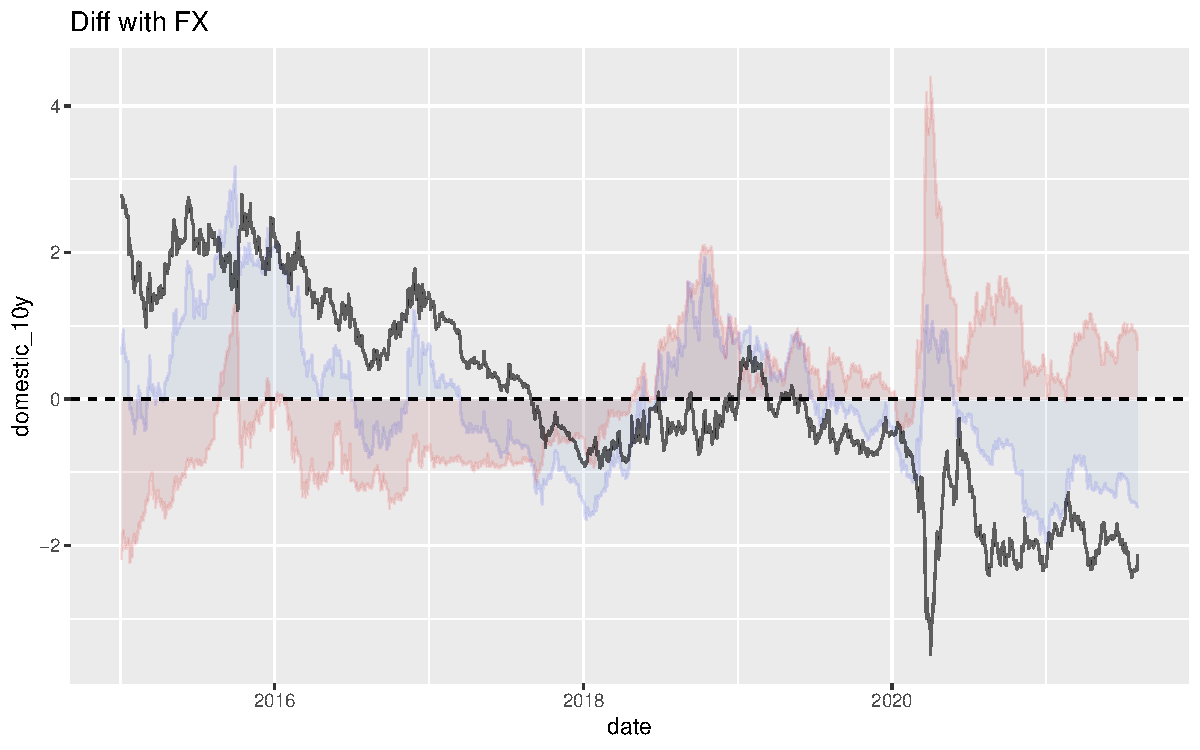
\includegraphics{Untitled_files/figure-latex/unnamed-chunk-24-3.pdf} 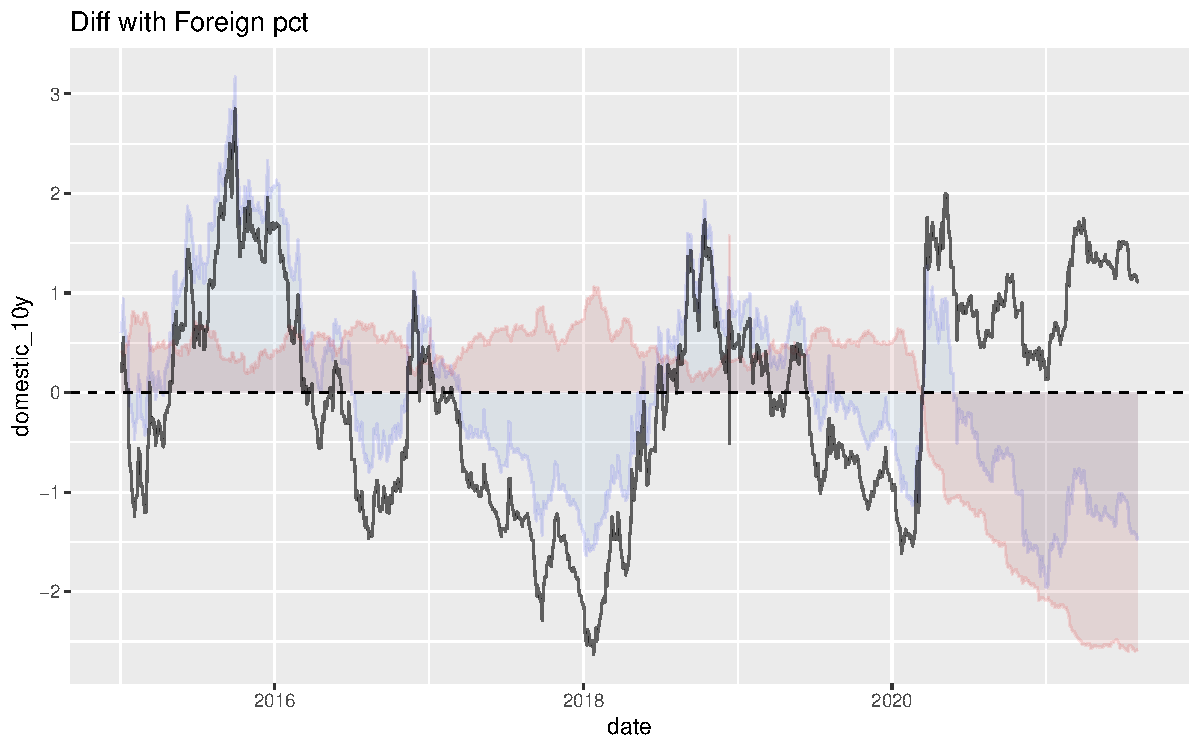
\includegraphics{Untitled_files/figure-latex/unnamed-chunk-24-4.pdf}

\begin{verbatim}
## Warning: Removed 338 rows containing missing values (position_stack).
\end{verbatim}

\begin{verbatim}
## Warning: Removed 338 row(s) containing missing values (geom_path).

## Warning: Removed 338 row(s) containing missing values (geom_path).
\end{verbatim}

\begin{verbatim}
## Warning: Removed 1 rows containing missing values (geom_hline).
\end{verbatim}

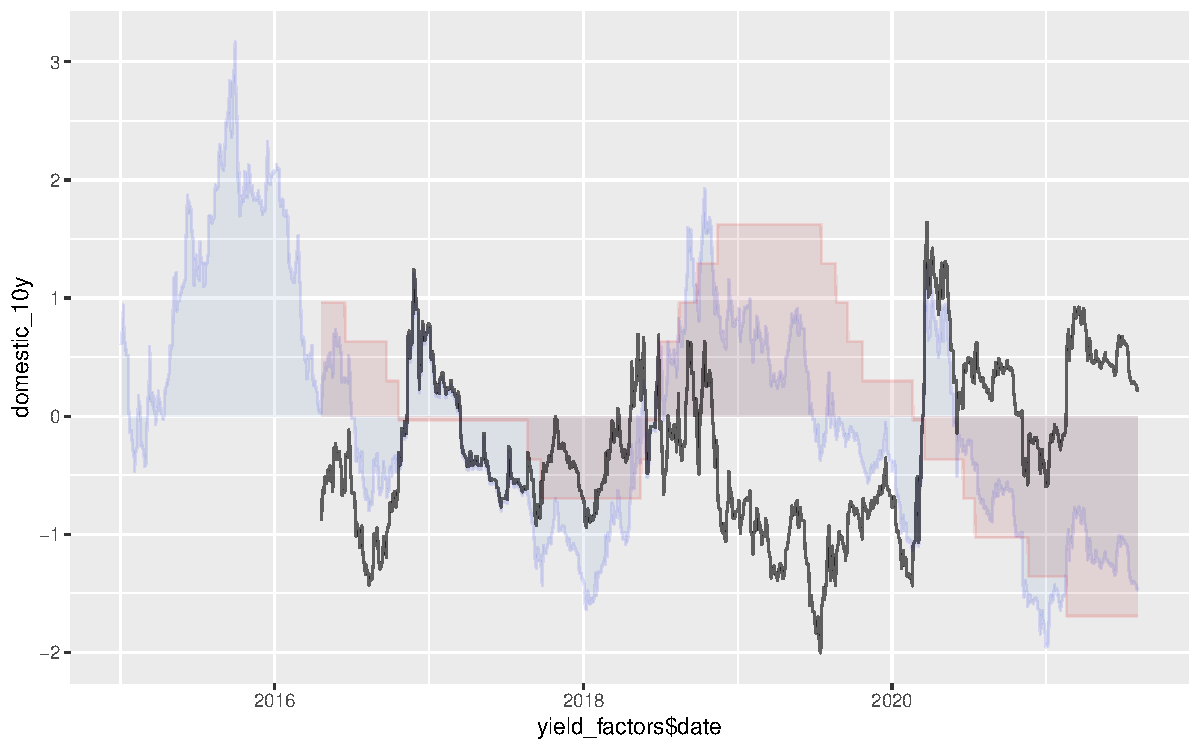
\includegraphics{Untitled_files/figure-latex/unnamed-chunk-24-5.pdf}

\begin{verbatim}
## Warning: Removed 3 rows containing missing values (position_stack).

## Warning: Removed 1 rows containing missing values (geom_hline).
\end{verbatim}

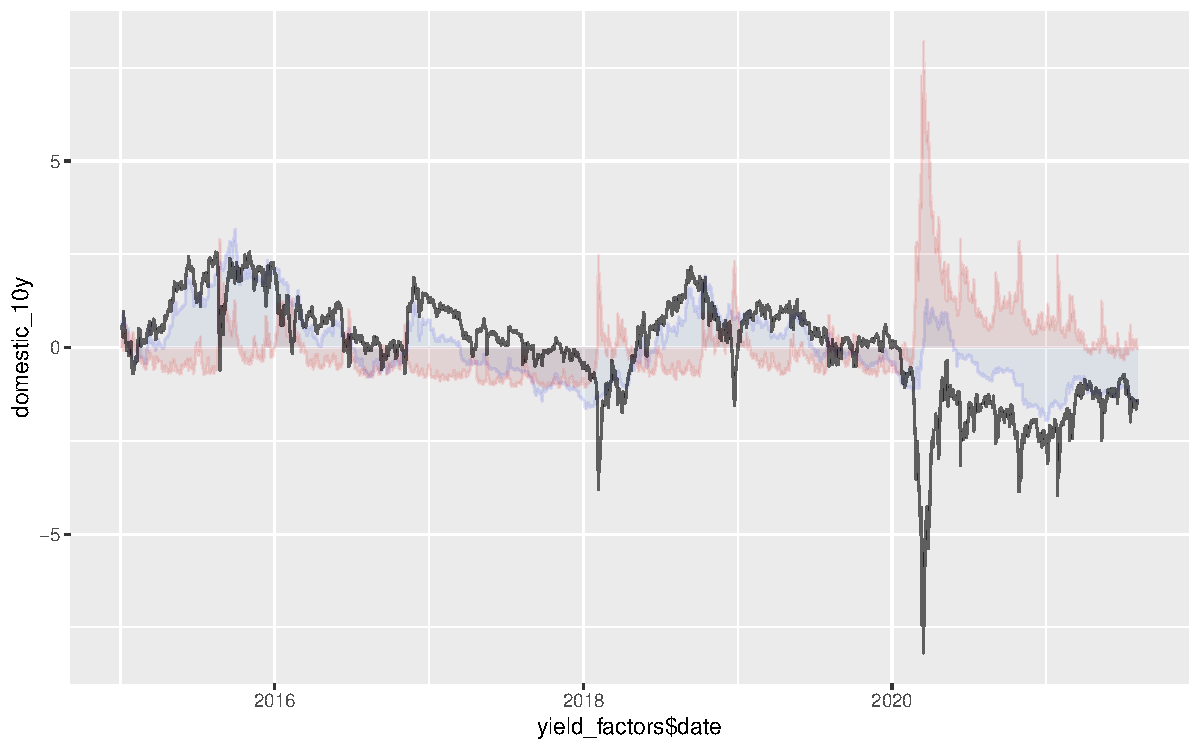
\includegraphics{Untitled_files/figure-latex/unnamed-chunk-24-6.pdf}

\hypertarget{formal-test}{%
\subsubsection{Formal Test}\label{formal-test}}

\hypertarget{linear-model}{%
\subsubsection{Linear Model}\label{linear-model}}

Regarding the result from the exploratory data analysis conducted in previous section as well as the cointegration test, we can write down relationship between variables in OLS model as follow:

\[
\begin{aligned}
yield\_10y = &\alpha + \beta_1ust\_10y+\beta_2cds\_5y +\beta_3foreign\_pct + \beta_4policy\_rate +\beta_5exchange\_rate
\\
&+ \beta_6{vix}^2 + \beta_7auction\_days +\epsilon
\end{aligned}
\]

Summary statistic of the data is shown in table \ref{tab:table1}:

\begin{table}[!htbp] \centering 
  \caption{} 
  \label{tab:table1} 
\begin{tabular}{@{\extracolsep{5pt}}lccccccc} 
\\[-1.8ex]\hline 
\hline \\[-1.8ex] 
Statistic & \multicolumn{1}{c}{N} & \multicolumn{1}{c}{Mean} & \multicolumn{1}{c}{St. Dev.} & \multicolumn{1}{c}{Min} & \multicolumn{1}{c}{Pctl(25)} & \multicolumn{1}{c}{Pctl(75)} & \multicolumn{1}{c}{Max} \\ 
\hline \\[-1.8ex] 
10y Yield & 1,371 & 7.165 & 0.612 & 5.886 & 6.673 & 7.650 & 8.878 \\ 
5y CDS & 1,371 & 115.163 & 38.156 & 58 & 85.3 & 137.6 & 291 \\ 
10y UST & 1,371 & 1.961 & 0.731 & 0.507 & 1.534 & 2.518 & 3.237 \\ 
Policy Rate & 1,371 & 4.776 & 0.754 & 3.500 & 4.250 & 5.250 & 6.000 \\ 
Foreign Pct & 1,371 & 0.354 & 0.056 & 0.225 & 0.324 & 0.389 & 0.442 \\ 
VIX & 1,371 & 17.796 & 8.562 & 9.140 & 12.420 & 20.740 & 82.690 \\ 
Exchange Rate & 1,371 & 14,006.420 & 625.921 & 12,926 & 13,400 & 14,417.5 & 16,741 \\ 
\hline \\[-1.8ex] 
\end{tabular} 
\end{table}

\hypertarget{analysis}{%
\section{Analysis}\label{analysis}}

In particular, the results suggest that
improved macroeconomic fundamentals, such as higher net foreign assets (in
terms of GDP or imports), lower fiscal deficits, and lower ratios of debt service to
exports and debt to GDP, help to lower sovereign spreads \textcite{arora}

\begin{enumerate}
\def\labelenumi{\alph{enumi}.}
\item
  UST vs Yield
  While the dramatic rise in capital flows to
  emerging markets has been induced primarily by the implementation of sound
  macroeconomic policies and wide structural reforms in these countries, it has
  also been driven by changing conditions in industrial countries that have
  encouraged investors to diversify their portfolios into developing country
  assets. Interest rate spreads (the differences between yields on
  sovereign bonds of developing countries and U.S. treasury securities of
  comparable maturities), which are a proxy for country risk, have tended to
  move in the same direction as the changes in U.S. interest rates \textcite{arora}
\item
  CDS vs Yield
\end{enumerate}

Sovereign CDS spreads are used as an indicator of foreign currency sovereign
creditworthiness. Lower sovereign CDS spreads are expected to lower local currency sovereign bond yields \textcite{gadanecz}

\begin{enumerate}
\def\labelenumi{\alph{enumi}.}
\setcounter{enumi}{2}
\item
  Foreign Ownership vs Yield
\item
  Bank Indo Rate vs Yield
\item
  Exchange rate (JISDOR) vs Yield
  Investors are exposed to gains and losses from exchange rate movements on their holdings of local currency sovereign bond. exchange rate risk can represent an important channel of transmission of market sentiment, uncertainty and default risk to local currency bond yield
  Exchange rate risk tends to affect liquidity
  conditions in both foreign exchange and domestic bond markets, which tend to be relatively low in many EMEs even in tranquil times.
  The direction of the
  causality runs from exchange rate volatility to local currency sovereign bond yields. This is especially the case in Asia and eastern
  Europe. In these two regions, local currency sovereign bond markets are relatively liquid and foreign participation relatively large.
\end{enumerate}

The sensitivity of EME local currency sovereign bond yields to exchange rate volatility increases after
the global financial crisis, and further after the taper tantrum in mid-2013
\textcite{gadanecz}

\begin{enumerate}
\def\labelenumi{\alph{enumi}.}
\setcounter{enumi}{5}
\tightlist
\item
  Volatility index (VIX) vs Yield
  It is a measure of market expectations of near-term volatility conveyed by S\&P500 stock index option prices and considered as a forward-looking measure of investor risk. Hartelius et al.~(2008) highlights the strong dependence of emerging market returns to the VIX, which should be positively
  related to changes in emerging market spreads since more risk aversion increases spreads. An attractive feature of this index is that it can
  be considered as exogenous for emerging economies (Siklos, 2011). \textcite{hajer}
\end{enumerate}

This result could be explained by the fact that as investors become more risk-averse and seek safer assets, the expected growth in volatility encourages them to liquidate their positions in risky assets in favor of safer ones, thus increasing sovereign spreads.
\textcite{hajer}

Intended to capture changes in investor sentiment which may be related to
expected changes in U.S. monetary policy. It may also pick up the effects of other market-related events, such as the flight to quality effects during the Asian crisis.
\textcite{arora}

As historical data demonstrates a strong negative correlation of volatility to the stock market returns -- that is, when stock returns go down, volatility rises and vice versa.(investopedia)

\hypertarget{conclusion}{%
\section{Conclusion}\label{conclusion}}

factors that steadily affect the yield? (foreign and insurance/pension fund are steadily associated with yield movement. Foreign has strongly negative correlation until 2019, while insurance/pension has strongly positive correlation)

pandemic effect? i.e.~holding spending for investing in safe instrument? (need to check ownership of domestic banks, mutual funds, insurance, individual investors)

shifting power (bonds ownership) foreign to domestic participant (Do central bank/domestic banks become more dominant)?
(Quantitative easing of Bank Indonesia and mandatory purchase of domestic banks can push down the yield)

As we can see from the plot, in 2015 and 2016 foreign ownership seems to have no strong relationship with the yield. Different situation happened in 2017-2019 where the changes in foreign ownership seems to strong-negatively affect the bonds yield movement.

To mention, 2017 is the year when Indonesia got investment grade rating from S\&P, following FITCH and Moody's in previous years. It means that broader category of foreign investment entities (i.e.~pension funds and insurance) can enter the country's market since Indonesia's rating has fulfilled their criteria of investment (yunianto, 2018).

Particularly In 2020, the pattern is quite anomaly in which increase from 0.25-0.33\% in foreign ownership seems to raise the yield from 6 up to 8.5\%. The yield stumbles afterwards with the increase of foreign ownership up to 40\%.

In January-August 2021, the relationship looks non-linear with no obvious pattern. The ownership drops below 25\% but interestingly yield decreases further (6-7\%).

We may assume that the anomaly in 2020 and 2021 are due to Covid19 pandemic that occurred since early 2020. The government is increasing its funding to sustain the economy. The decrease in foreign portion could be because foreigners sell their bonds more than their buying (net sell), or another reason is because their portion is deluged by domestic participants (i.e.~central bank), thus we will track the pattern of domestic ownership in these years to check our assumption.

\begin{verbatim}
## 
## Call:
## lm(formula = domestic_10y ~ cds_5y + ust_10y + foreign + rate + 
##     con_bank, data = yield_factors)
## 
## Residuals:
##      Min       1Q   Median       3Q      Max 
## -1.44899 -0.15056 -0.03247  0.17758  0.75192 
## 
## Coefficients:
##              Estimate Std. Error t value Pr(>|t|)    
## (Intercept) 1.477e+00  9.800e-02   15.07   <2e-16 ***
## cds_5y      1.171e-02  2.492e-04   47.01   <2e-16 ***
## ust_10y     3.056e-01  1.252e-02   24.40   <2e-16 ***
## foreign     1.082e-03  7.989e-05   13.55   <2e-16 ***
## rate        4.955e-01  1.382e-02   35.85   <2e-16 ***
## con_bank    6.016e-04  3.615e-05   16.64   <2e-16 ***
## ---
## Signif. codes:  0 '***' 0.001 '**' 0.01 '*' 0.05 '.' 0.1 ' ' 1
## 
## Residual standard error: 0.2404 on 1368 degrees of freedom
##   (338 observations deleted due to missingness)
## Multiple R-squared:  0.8461, Adjusted R-squared:  0.8456 
## F-statistic:  1504 on 5 and 1368 DF,  p-value: < 2.2e-16
\end{verbatim}

\begin{verbatim}
## `geom_smooth()` using method = 'gam'
## `geom_smooth()` using method = 'gam'
## `geom_smooth()` using method = 'gam'
## `geom_smooth()` using method = 'gam'
## `geom_smooth()` using method = 'gam'
\end{verbatim}

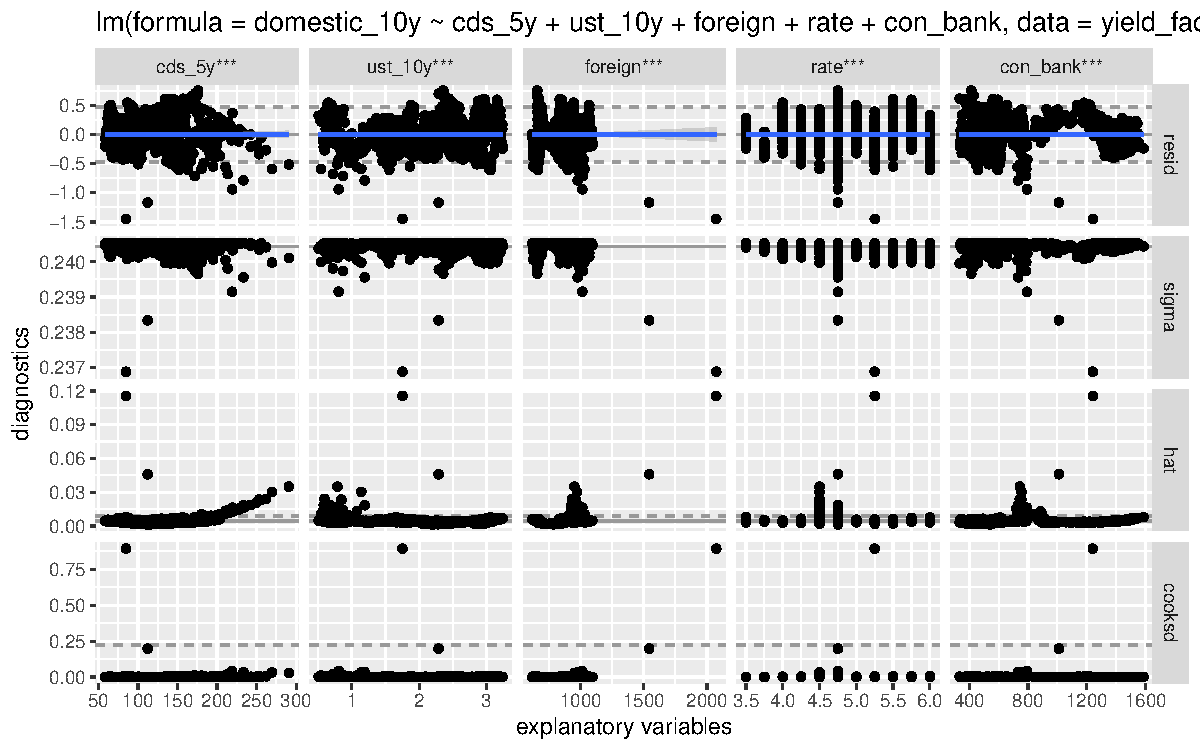
\includegraphics{Untitled_files/figure-latex/unnamed-chunk-28-1.pdf}

As shown in the plot, proportion of Bank Indonesia and Conventional Bank are getting bigger in 2020-2021, while proportion of foreign holders is diluted. This is can be seen as a result of implementation of new regulation on 1 May 2020 that mandate banks to reserve government bonds. This regulation has an impact on reducing bonds yield further in these two consecutive years.

Another noticeable change is proportion of individual in the bonds ownership that is growing started from mid of 2020 up to 2021. We may argue that people who prefer to hold their spending is channelling their excess money to investment, especially in a safe instrument like government bonds.

\hypertarget{policy-rate}{%
\subsection{Policy Rate}\label{policy-rate}}

From plot above, the movement of domestic 10y yield is parallel with movement of policy rate. The median spread in 2016 until 2018 is quite the same (around 2.5) while median spread of 2019 is the lowest. In 2020 and 2021, the differences between 10y yield and policy rate are increase with median spread is about 3. The range of spread in 2020 is also the widest compared to other observed years.

\printbibliography[title=Bibliography]

\end{document}
